\documentclass[11pt]{article}

\usepackage[T1]{fontenc}
\usepackage[utf8]{inputenc}
\usepackage[a4paper, margin=1in]{geometry}
\usepackage{lmodern}
\usepackage{float}
\usepackage{amsmath, amssymb, booktabs, array, graphicx}
\usepackage{natbib}
\usepackage{url}
\usepackage[colorlinks = true, linkcolor = blue, citecolor = blue, urlcolor = blue]{hyperref}

\newcommand{\appname}{Partial Association Explorer}
\newcolumntype{L}[1]{>{\raggedright\arraybackslash}p{#1}}
\newcommand{\code}[1]{\texttt{#1}}
\newcommand{\pkg}[1]{\textsf{#1}}
\newcommand{\proglang}[1]{\textsf{#1}}
\newcommand{\email}[1]{\href{mailto:#1}{#1}}
\newcommand{\doi}[1]{\href{https://doi.org/#1}{doi:#1}}

\author{
  Thadd\'ee D'haegeleer\textsuperscript{a},
  C\'edric Heuchenne\textsuperscript{a,b},
  Antoine Soetewey\textsuperscript{a,b}\\[0.6em]
  \normalsize\textsuperscript{a} CAPE, UCLouvain Saint-Louis Bruxelles\\
  \normalsize\textsuperscript{b} HEC Li\`ege, Universit\'e de Li\`ege\\[0.4em]
  \normalsize Corresponding author: \email{thaddee.dhaegeleer@uclouvain.be}
}

\title{\appname: Interactive Profiling of Marginal and Conditional Associations in Mixed-Type Data}
\date{}

\begin{document}

\maketitle

\begin{abstract}
  \appname{} is an open-source \proglang{R} \citep{R} \pkg{shiny}
  \citep{Shiny} application for exploratory association analysis in datasets
  containing both numerical and categorical variables. The software computes a
  global association measure, a formal significance test, and a local pairwise
  diagnostic for every selected variable pair. Three pair types are handled in
  a unified workflow: numerical--numerical, numerical--categorical, and
  categorical--categorical. A central feature of the application is the
  possibility of selecting control variables and recomputing the full
  association structure conditionally, allowing users to distinguish marginal
  relationships from associations that remain after adjustment, disappear as
  likely spurious links, or emerge only once a masking background variable has
  been taken into account. The interface combines filtered association
  networks, harmonized pair plots, exportable summaries, and likelihood-based
  diagnostics for categorical pairs. This article describes the statistical
  framework implemented in the software, the main design and optimization
  choices underlying the app, and an illustrative analysis workflow
  based on survey data.
\end{abstract}

\noindent\textbf{Keywords:} \proglang{R}, \pkg{shiny}, exploratory data analysis, mixed-type data, conditional association, likelihood-ratio tests, association network.

\bigskip

\section[Introduction: Association profiling in R]{Introduction: Association profiling in \proglang{R}}
\label{sec:intro}

Exploratory analysis often begins with a simple question: which variables in a
dataset are associated? In practice, this question becomes substantially harder
when the data mix numerical and categorical variables and when plausible
confounders should be taken into account. Classical correlation matrices cover
only numerical variables, while standard contingency-table summaries do not
provide a unified treatment of mixed pair types. Even when pairwise summaries
exist, marginal associations can be misleading if two variables are jointly
related to age, education, region, time, or another background factor.

\appname{} addresses this problem as a software workflow rather than as a
single statistical test. It provides a guided interface for computing and
visualizing both \emph{global} and \emph{local} associations between all
selected pairs of variables. Global association is the single strength measure
used to draw and filter the network, while a companion significance test
provides a $p$-value for the corresponding null hypothesis. Local association
is the observation-, group-, or cell-level diagnostic shown in the pair plots.
The same application handles the unconditional case and the conditional case,
where users select control variables $Z$ before recomputing the association
network. Importantly, the interface keeps the same logic across pair types: one
global measure for filtering, one formal test for significance, and one local
plot explaining the edge, whether the user is looking at the raw structure or
at the adjusted one.

The application builds on \pkg{AssociationExplorer}
\citep{SoeteweyHeuchenneClaesDescampe2026}, which showed how an accessible
\pkg{shiny} interface can lower the barrier to marginal association exploration
in mixed-type data. \appname{} extends that workflow in three main directions.
First, it adds conditional association analysis through a common control-variable
interface applied across all pair types. Second, it performs a formal test of
association for every selected pair rather than reporting effect sizes alone.
Third, it expands the local visual diagnostics, especially for
categorical--categorical pairs, where the software relies on likelihood-based
global measures and residual-based local displays.

The intended audience is broader than a purely methodological readership. In
social-science and economic applications, users often begin with a long list of
survey items, behavioural indicators, institutional variables, and demographic
controls, and the first challenge is to understand which relationships deserve
closer study. \appname{} is useful precisely because it helps users move beyond
raw pairwise description. An unconditional screening can be followed by the
same analysis with controls to determine whether an edge remains, disappears as
a likely confounded association, or becomes visible only after adjustment
because a background variable was masking it. In that sense, the application is
not only a visualization layer but a practical exploratory tool for separating
descriptively visible, spurious, and hidden associations in mixed-type data.
This unconditional--conditional comparison is especially valuable for applied
users because it turns a potentially technical adjustment exercise into a
transparent, clickable comparison of two network views and their corresponding
pair plots.

From a statistical perspective, the three pair types are handled by matched
global measures and tests: Pearson's $r$ and partial $r$ for
numerical--numerical pairs, $\eta^2$ and partial $\eta^2$ for
numerical--categorical pairs, and likelihood-ratio-based coefficients $V_L$
and $V_{L\mid Z}$ for categorical--categorical pairs. All measures are
described in Section~\ref{sec:framework}, and additional computational details
are collected in the appendix.

The remainder of the article is organized as follows. Section~\ref{sec:overview}
describes the software workflow and outputs. Section~\ref{sec:framework}
presents the implemented statistical framework for all pair types.
Section~\ref{sec:implementation} details the most important implementation and
optimization choices in the app. Section~\ref{sec:example} gives an
illustrative workflow showing how the software can both remove a confounded
association and reveal a hidden one. Section~\ref{sec:related} situates the app
relative to related software, and Section~\ref{sec:discussion} concludes with
strengths, limitations, and possible extensions. Additional mathematical
details are collected in the appendix.

\section{Software overview and workflow}
\label{sec:overview}

\appname{} is a standalone \pkg{shiny} application distributed through a public
GitHub repository. Users upload a \code{.csv}, \code{.xls}, or \code{.xlsx}
file and may optionally upload a two-column variable-description file. The
software then:

\begin{enumerate}
  \item removes variables whose non-missing values take only a single distinct
    value;
  \item detects pair types from the imported \proglang{R} classes, treating
    variables for which \code{is.numeric()} is true as numerical and the others
    as categorical;
  \item lets the user choose analysis variables and optional control variables;
  \item computes all pairwise associations, associated tests, and local
    diagnostics;
  \item displays the retained associations in a filtered network;
  \item allows the user to inspect each retained edge through pair plots.
\end{enumerate}

Selected analysis variables appear as nodes in the association network. Control
variables are used for adjustment but do not appear as nodes. Thresholds are
applied after all pairwise quantities have been computed: the user can filter
numerical--numerical and numerical--categorical edges by a range for $R^2$ or
$\eta^2$, categorical--categorical edges by a range for $V_L$, and all edges
by a range of $p$-values. When controls are selected, the app can also display
the conditional network together with a visual comparison to the corresponding
unconditional view. The user can switch the displayed network from the
unconditional structure to the conditional one and back again. In that
comparison mode, the edge colours are interpreted relative to the specific view
that is currently shown: green edges are present only in the displayed view,
whereas muted grey dotted edges belong only to the alternative view and are
shown for comparison.

The core workflow is summarized in Table~\ref{tab:measures}. The software uses
different statistical models depending on the pair type, but the outputs are
deliberately harmonized: each pair receives one global association measure, one
formal test, and one local plot adapted to the data type.

\begin{figure}[H]
\centering
\begin{minipage}{0.48\linewidth}
\centering
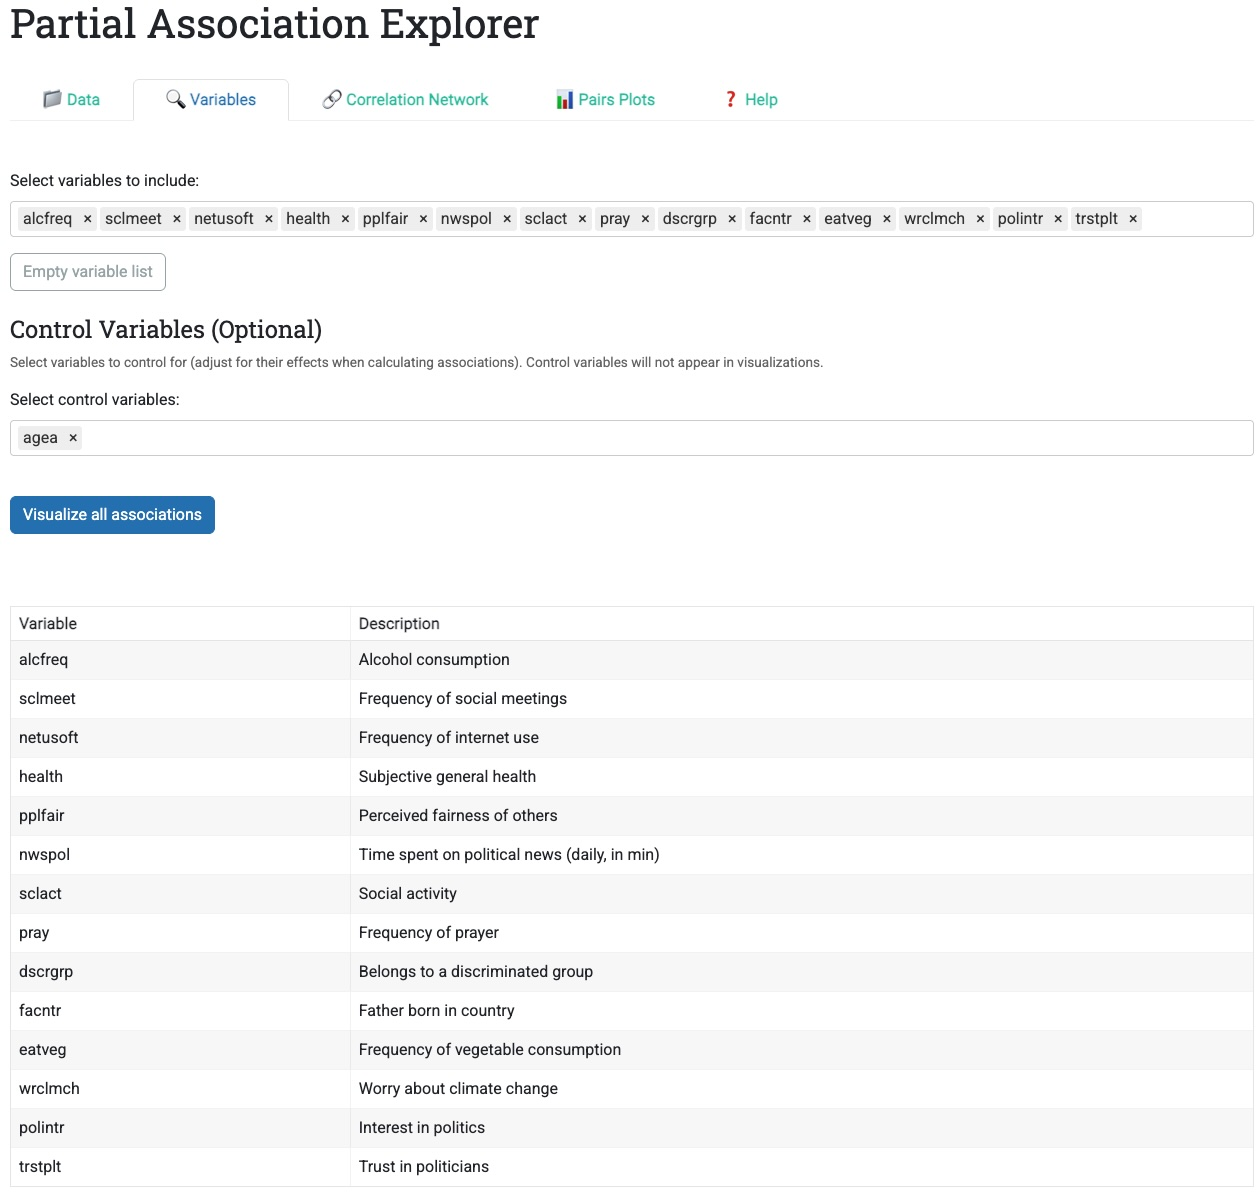
\includegraphics[width=\linewidth]{section2_variable_selection.jpg}
\par\smallskip
\small Variable and control selection.
\end{minipage}
\hfill
\begin{minipage}{0.48\linewidth}
\centering
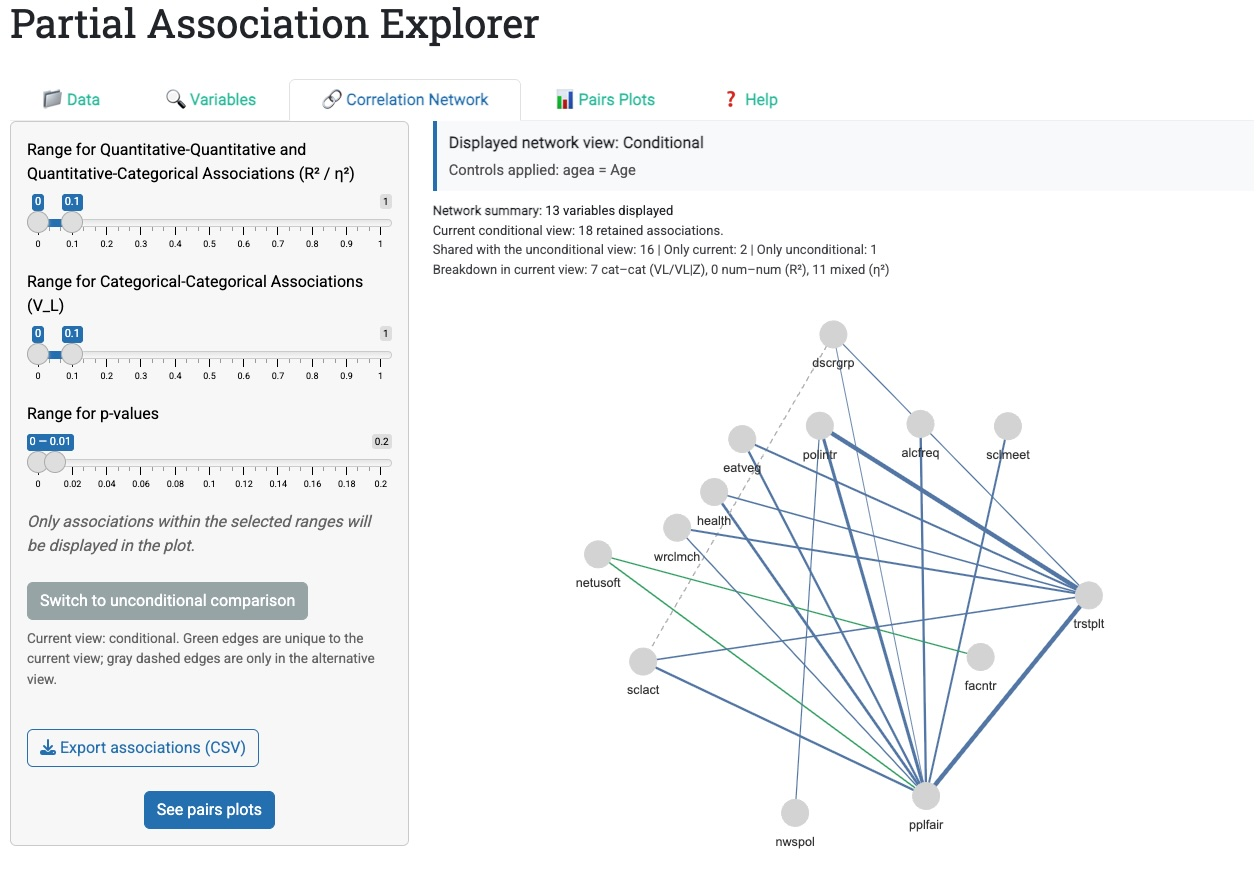
\includegraphics[width=\linewidth]{section2_network.jpg}
\par\smallskip
\small Filtered association network.
\end{minipage}
\caption{\label{fig:overviewshots} Workflow screens from \appname{} using the
2011 Belgian wave of the European Social Survey. The interface moves from
variable selection to a filtered network of retained associations.}
\end{figure}

\begin{table}[t!]
\centering
\setlength{\tabcolsep}{7pt}
\renewcommand{\arraystretch}{1.35}
\begin{tabular}{@{}L{3.15cm}L{3.35cm}L{3.55cm}L{3.05cm}@{}}
\toprule
Pair type & Unconditional measure and test & Conditional measure and test & Local pair plot \\
\midrule
Numerical--numerical &
Pearson's $r$ and a $t$-test &
Partial $r$ and a partial-correlation $t$-test &
Scatter plot or added-variable plot \\
Numerical--categorical &
$\eta^2$ and an ANOVA $F$-test &
Partial $\eta^2$ and an extra-sum-of-squares $F$-test &
Group means or residualized group means \\
Categorical--categorical &
$V_L$ and a likelihood-ratio $\chi^2$ test &
$V_{L\mid Z}$ and a conditional likelihood-ratio $\chi^2$ test &
Contingency table with observed counts and Pearson residuals \\
\bottomrule
\end{tabular}
\caption{\label{tab:measures} Global association measures, significance tests,
and local pair plots implemented in \appname{}.}
\end{table}

Beyond the network and pair-plot views, the app also offers several
quality-of-life features that are useful in practice: variable descriptions can
be displayed throughout the interface, retained pairwise summaries can be
exported as \code{.csv}, and when controls are selected the pair-plot panel can
show the conditional plot together with its unconditional counterpart so that
the effect of adjustment can be inspected visually.

\section{Implemented statistical framework}
\label{sec:framework}

\subsection{Numerical--numerical associations}
\label{sec:numnum}

Let $X$ and $Y$ be numerical variables observed on $n$ units. Without controls,
the software summarizes the association by Pearson's correlation coefficient
\begin{equation}
r_{XY} =
\frac{\sum_{t=1}^{n} (X_t - \bar{X})(Y_t - \bar{Y})}
{\sqrt{\sum_{t=1}^{n}(X_t - \bar{X})^2}
 \sqrt{\sum_{t=1}^{n}(Y_t - \bar{Y})^2}},
\label{eq:pearson}
\end{equation}
and filters the network on the corresponding $R^2 = r_{XY}^2$. The null
hypothesis $H_0: r_{XY} = 0$ is tested with the usual statistic
\begin{equation}
t = r_{XY}\sqrt{\frac{n-2}{1-r_{XY}^2}},
\label{eq:t-pearson}
\end{equation}
which is compared to a Student distribution with $n-2$ degrees of freedom.

With controls $Z = (Z_1, \dots, Z_q)$, the app computes a partial correlation
through the added-variable principle. Specifically, $X$ and $Y$ are separately
regressed on $Z$ and the resulting residuals $\tilde{X}$ and $\tilde{Y}$ are
correlated:
\begin{equation}
r_{XY\cdot Z} = \mathrm{cor}(\tilde{X}, \tilde{Y}).
\label{eq:partial-r}
\end{equation}
Again the network is filtered by the squared quantity $R^2_{XY\cdot Z}$.
Under $H_0: r_{XY\cdot Z} = 0$, the test statistic is
\begin{equation}
t = r_{XY\cdot Z}\sqrt{\frac{n-q-2}{1-r_{XY\cdot Z}^2}},
\label{eq:t-partial}
\end{equation}
with $n-q-2$ degrees of freedom.

The associated pair plots are designed to keep the interpretation stable across
cases. Without controls, the local display is a scatter plot with fitted linear
trend. With controls, it becomes an added-variable plot, that is, a scatter
plot of the residuals of $X$ and $Y$ after removing the linear contribution of
$Z$. Additional computational details for the unconditional and conditional
numerical--numerical cases are collected in Appendix~\ref{app:numnum}
(p.~\pageref{app:numnum}).

Reading these plots is direct. In the unconditional panel, the slope and the
overall cloud summarize the marginal association: an upward fitted line means
that larger values of one variable tend to go with larger values of the other.
In Figure~\ref{fig:numnumshots}, the positive pattern suggests that respondents
who give higher answers on perceived fairness also tend to report greater trust
in politicians. In the conditional panel, the same reading applies to the
residualized variables: the slope now reflects the remaining association after
the linear effect of the control has been removed from both axes.

\begin{figure}[H]
\centering
\begin{minipage}{0.48\linewidth}
\centering
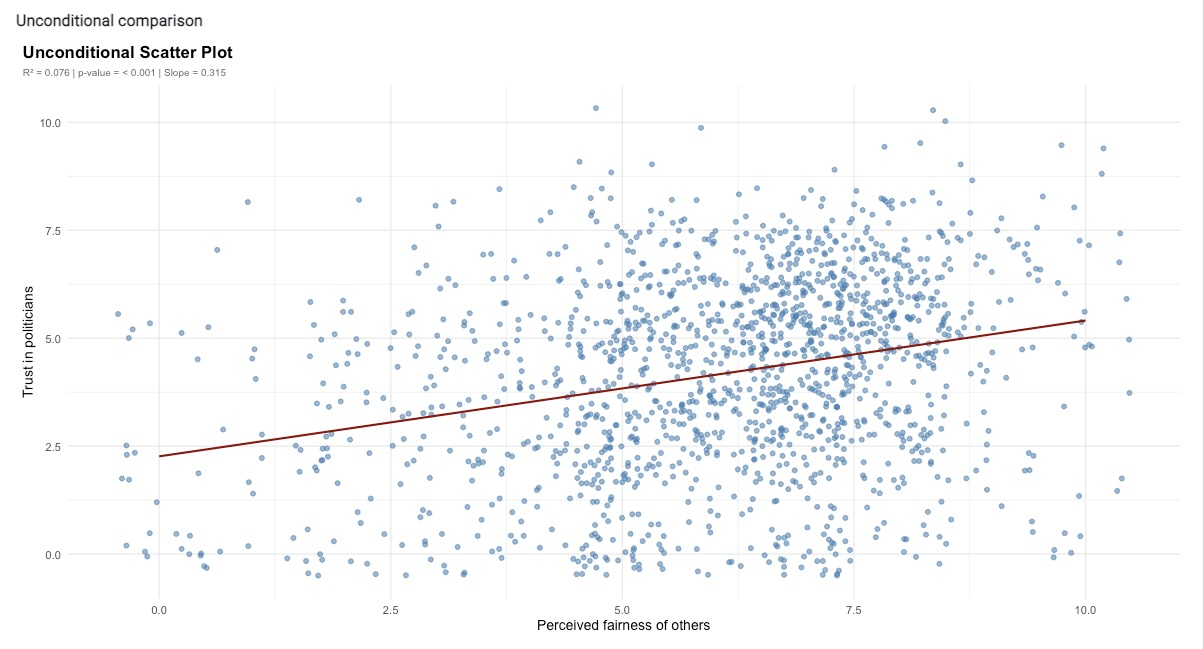
\includegraphics[width=\linewidth]{section3.1_unconditional_pairplot_pplfair_trstplt.jpg}
\par\smallskip
\small Unconditional pair plot.
\end{minipage}
\hfill
\begin{minipage}{0.48\linewidth}
\centering
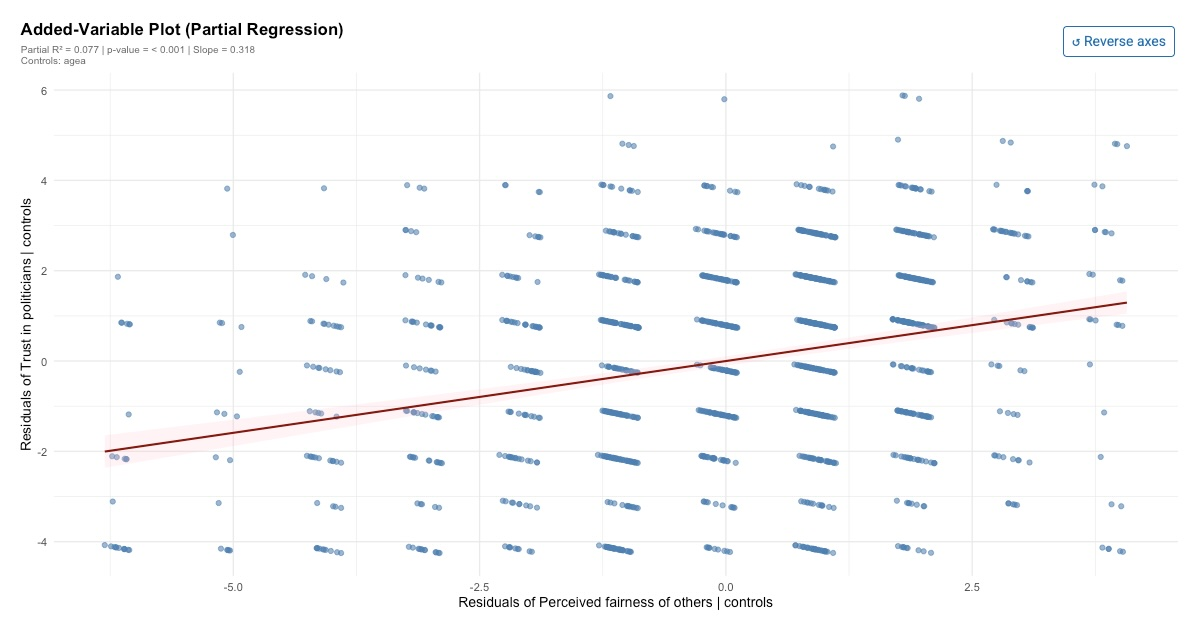
\includegraphics[width=\linewidth]{section3.1_conditional_pairplot_pplfair_trstplt_agea.jpg}
\par\smallskip
\small Conditional pair plot with age of respondent (\code{agea}) as control.
\end{minipage}
\caption{\label{fig:numnumshots} Illustrative numerical--numerical pair plots
from the 2011 Belgian ESS for perceived fairness of others (\code{pplfair})
and trust in politicians (\code{trstplt}). The conditional version replaces
the raw scatter with the added-variable view used to compute the partial
association after adjusting for age of respondent (\code{agea}).}
\end{figure}

\subsection{Numerical--categorical associations}
\label{sec:numcat}

Let $Y$ be numerical and let $X$ be categorical with $J$ groups. In the
unconditional case, the software uses the classical ANOVA effect size
\begin{equation}
\eta^2 = \frac{\mathrm{SSB}}{\mathrm{SST}},
\label{eq:eta2}
\end{equation}
where $\mathrm{SSB}$ is the between-group sum of squares and $\mathrm{SST}$ is
the total sum of squares. The null hypothesis of equal group means is tested by
the usual ANOVA statistic
\begin{equation}
F = \frac{\mathrm{SSB}/(J-1)}{\mathrm{SSW}/(n-J)},
\label{eq:f-anova}
\end{equation}
with $\mathrm{SSW}$ denoting the within-group sum of squares.

With controls, the app uses an ANCOVA/extra-sum-of-squares construction. A
reduced model
\begin{equation}
Y_t = \alpha' + \sum_{k=1}^{q}\gamma'_k Z_{kt} + \varepsilon'_t
\label{eq:red-model}
\end{equation}
is compared to a full model
\begin{equation}
Y_t = \alpha + \sum_{j=2}^{J}\beta_j \mathbf{1}\{X_t = j\}
      + \sum_{k=1}^{q}\gamma_k Z_{kt} + \varepsilon_t.
\label{eq:full-model}
\end{equation}
If $\mathrm{RSS}_{red}$ and $\mathrm{RSS}_{full}$ are the residual sums of
squares, the software reports
\begin{equation}
\eta^2_{X\mid Z} =
\frac{\mathrm{RSS}_{red} - \mathrm{RSS}_{full}}
     {(\mathrm{RSS}_{red} - \mathrm{RSS}_{full}) + \mathrm{RSS}_{full}},
\label{eq:partial-eta}
\end{equation}
which is equivalent to the proportion of the residual variation left after
adjusting for $Z$ that is further explained by the group structure induced by
$X$. The corresponding $F$-test is
\begin{equation}
F =
\frac{(\mathrm{RSS}_{red} - \mathrm{RSS}_{full})/(J-1)}
     {\mathrm{RSS}_{full}/\mathrm{df}_{full}}.
\label{eq:f-ancova}
\end{equation}

The pair plots again follow a common logic. Without controls, the local display
is a group-means plot of the raw outcome. With controls, the software first
fits $Y$ on $Z$, extracts residuals
\begin{equation}
\tilde{Y}_t = Y_t - \widehat{E}(Y_t \mid Z_t),
\label{eq:yresid}
\end{equation}
and then plots the group means of $\tilde{Y}$ across the categories of $X$.
These residualized means show the remaining group differences after removing
the linear contribution of the controls. Explicit computational formulas,
including the definitions of $\mathrm{SSB}$, $\mathrm{SST}$, $\mathrm{SSW}$,
and the residualized-means construction, are collected in
Appendix~\ref{app:numcat} (p.~\pageref{app:numcat}).

These plots should be read vertically. Without controls, the displayed points
or bars are raw group means. With controls, they are means of residualized
values, so positive or negative positions indicate above- or below-expected
levels of the numerical outcome after adjustment rather than positive or
negative outcome values in an absolute sense. In
Figure~\ref{fig:numcatshots}, differences across alcohol-frequency groups show
how average responses on perceived fairness vary marginally and, in the
conditional panel, how much of that variation remains once age has been taken
into account.

Figure~\ref{fig:numcatshots} also shows how the printed numbers should be read.
In the unconditional panel, they are raw group means: respondents who report
drinking several times a week have an average perceived fairness score of 6.39,
whereas respondents who never drink have an average of 5.58. In the
conditional panel, the numbers are no longer raw means but group averages of
the residualized outcome after removing the linear effect of age. The zero line
therefore represents the fairness level predicted by age alone. A value of
$0.32$ for ``Several times a week'' means that this group scores on average
about 0.32 points above its age-predicted level, whereas the value around
$-0.48$ for ``Never'' means that abstainers score about half a point below what
would be expected given their age. Negative bars do not indicate negative
fairness scores; they indicate below-expected fairness once age has been
removed. In this example, the ordering remains broadly similar before and after
adjustment, which suggests that age contributes to the pattern but does not
fully explain it.

\begin{figure}[H]
\centering
\begin{minipage}{0.48\linewidth}
\centering
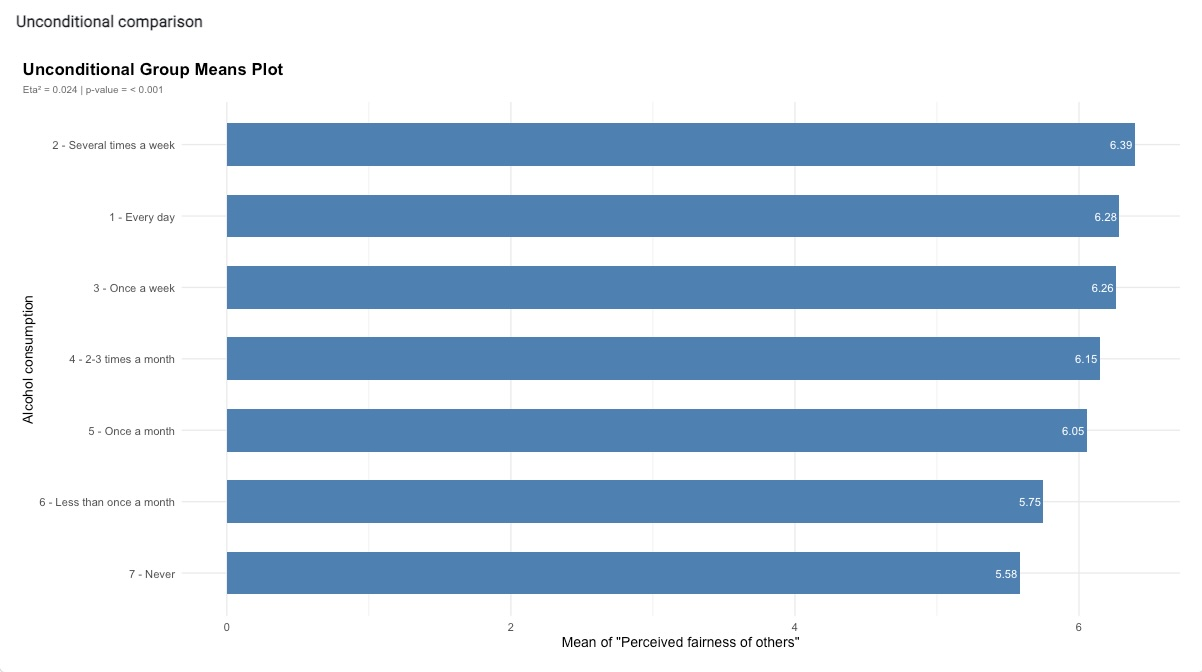
\includegraphics[width=\linewidth]{section3.2_unconditional_pairplot_alcfreq_pplfair.jpg}
\par\smallskip
\small Unconditional pair plot.
\end{minipage}
\hfill
\begin{minipage}{0.48\linewidth}
\centering
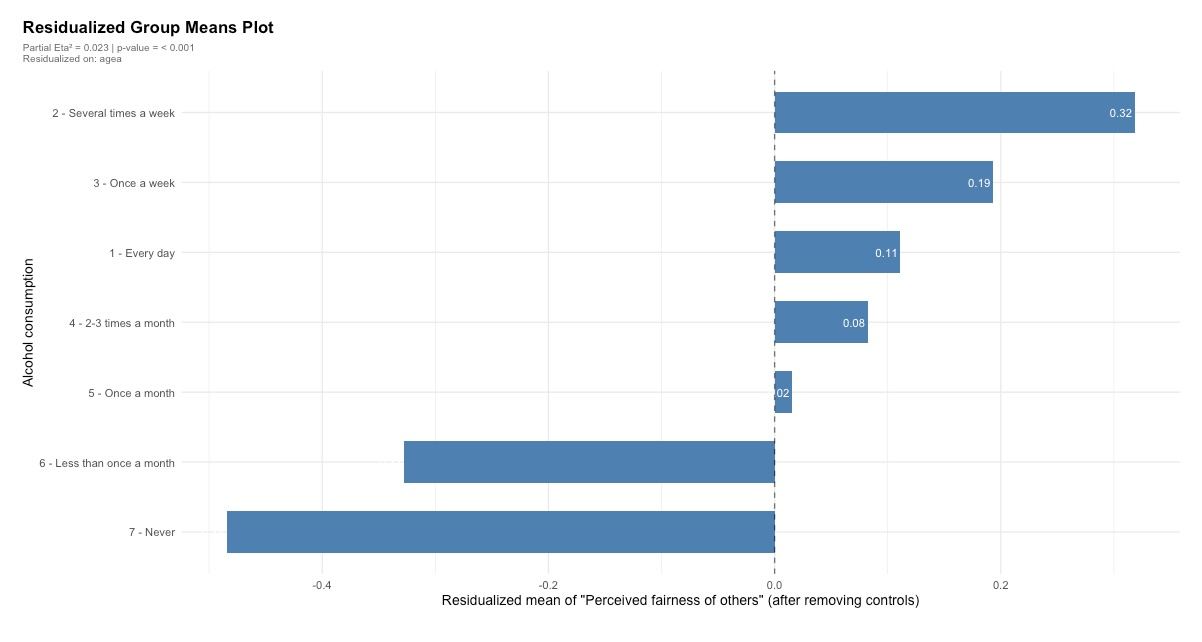
\includegraphics[width=\linewidth]{section3.2_conditional_pairplot_alcfreq_pplfair_agea.jpg}
\par\smallskip
\small Conditional pair plot with age of respondent (\code{agea}) as control.
\end{minipage}
\caption{\label{fig:numcatshots} Illustrative numerical--categorical pair plots
from the 2011 Belgian ESS for perceived fairness of others (\code{pplfair}) by
frequency of alcohol consumption (\code{alcfreq}). The conditional view
displays residualized group means after removing the linear contribution of age
of respondent (\code{agea}).}
\end{figure}

\subsection{Categorical--categorical associations}
\label{sec:catcat}

For categorical variables $X$ and $Y$ with $I$ and $J$ levels, respectively,
the software treats the pair $(X,Y)$ as a single joint categorical outcome
$W = (X,Y)$ with $K = IJ$ categories. The modelling strategy is based on
baseline-category multinomial logits relative to the first cell.

When controls are present, let $Z = (Z_1, \dots, Z_q)$ denote the control
vector after model-matrix coding of categorical controls. Under the null model
of conditional independence, the linear predictor for cell $(i,j)$ is
\begin{equation}
\eta^{(0)}_{ij}(z)
=
\alpha_i + \beta_j + \lambda_i^\top z + \kappa_j^\top z,
\label{eq:eta0}
\end{equation}
whereas the alternative model adds an interaction term:
\begin{equation}
\eta^{(1)}_{ij}(z)
=
\alpha_i + \beta_j + \lambda_i^\top z + \kappa_j^\top z + \gamma_{ij}.
\label{eq:eta1}
\end{equation}
The unconditional case is obtained by dropping the $z$-dependent terms.

The terms in these predictors have a direct interpretation. The parameters
$\alpha_i$ and $\beta_j$ are category-specific baseline effects for the levels
of $X$ and $Y$: $\alpha_i$ shifts the logit for row category $i$ of $X$, while
$\beta_j$ shifts the logit for column category $j$ of $Y$. The term
$\lambda_i^\top z$ is the contribution of the control vector $z$ to row
category $i$, and $\kappa_j^\top z$ is the analogous control contribution to
column category $j$. Under the null model, these terms allow the controls to
change the fitted margins of $X$ and $Y$ without introducing any residual
association between them. The interaction parameter $\gamma_{ij}$, present only
in the alternative model, captures the remaining cell-specific association
after accounting for these main effects and control contributions. The symbol
$\delta$ is used later in the appendix for a different purpose, namely the
control slopes in the residualization regression for numerical--categorical
pair plots.

The implementation uses reference-category constraints. If the first level of
$X$ and the first level of $Y$ are taken as baseline categories, then
\begin{equation}
\alpha_1 = \beta_1 = 0,
\qquad
\lambda_1 = \mathbf{0},
\qquad
\kappa_1 = \mathbf{0},
\qquad
\gamma_{1j} = \gamma_{i1} = 0.
\label{eq:constraints}
\end{equation}
The corresponding probabilities are
\begin{equation}
\pi^{(m)}_{ij}(z;\theta) =
\frac{\exp(\eta^{(m)}_{ij}(z))}
{\sum_{r=1}^{I}\sum_{s=1}^{J}\exp(\eta^{(m)}_{rs}(z))},
\qquad m \in \{0,1\},
\label{eq:pi}
\end{equation}
with the baseline cell receiving linear predictor zero.

For $m \in \{0,1\}$, the observation-level log-likelihood is
\begin{equation}
\ell_m(\theta) =
\sum_{t=1}^{n}\sum_{i=1}^{I}\sum_{j=1}^{J}
\mathbf{1}\{X_t=i, Y_t=j\}
\log \pi^{(m)}_{ij}(Z_t;\theta).
\label{eq:loglik}
\end{equation}
Let $\widehat{\theta}_0$ and $\widehat{\theta}_1$ denote the maximizers of
$\ell_0$ and $\ell_1$, and write $\ell_0 = \ell_0(\widehat{\theta}_0)$ and
$\ell_1 = \ell_1(\widehat{\theta}_1)$. The unconditional likelihood-ratio
deviance is
\begin{equation}
G^2 = 2(\ell_1 - \ell_0),
\label{eq:g2}
\end{equation}
which the app transforms into the bounded association measure
\begin{equation}
V_L = \sqrt{1 - \exp(-G^2/n)}.
\label{eq:vl}
\end{equation}
With controls, the same construction is applied to the nested conditional
multinomial models; if $G^2_{\mid Z}$ denotes the likelihood-ratio deviance
for that conditional comparison, the app reports
\begin{equation}
V_{L\mid Z} = \sqrt{1 - \exp(-G^2_{\mid Z}/n)}.
\label{eq:vlz}
\end{equation}
In the unconditional contingency-table case, $G^2/n$ is twice the empirical
mutual information between $X$ and $Y$ when natural logarithms are used.
Hence, $V_L$ is the sample analogue of Linfoot's informational coefficient of
correlation \citep{Linfoot1957}; related information measures for contingency
tables were discussed by \citet{HamdanTsokos1971}. The same transformation is
also the square root of a Cox--Snell likelihood-based coefficient of
determination \citep{CoxSnell1989}, related to pseudo-$R^2$ measures used in
discrete-choice and generalized linear modelling \citep{McFadden1974,
Nagelkerke1991}. This mutual-information identity is specific to the
unconditional table; once controls are introduced as regression covariates, the
same likelihood-ratio logic remains, but there is no equally simple
contingency-table formula.

Under regularity conditions, the associated significance test compares $G^2$
or $G^2_{\mid Z}$ to a $\chi^2$ distribution with
\begin{equation}
\mathrm{df} = (I-1)(J-1),
\label{eq:df}
\end{equation}
that is, the number of free interaction parameters.

The fitted null model also yields expected counts
\begin{equation}
\widehat{E}^{(0)}_{ij}
=
\sum_{t=1}^{n}\Pr(X=i, Y=j \mid Z_t; \widehat{\theta}_0)
=
\sum_{t=1}^{n}\pi^{(0)}_{ij}(Z_t; \widehat{\theta}_0),
\label{eq:e0}
\end{equation}
which reduce to the familiar independence expectations in the unconditional
contingency-table case. Further computational details for the multinomial
likelihood, expected counts, and local diagnostics are collected in
Appendix~\ref{app:catcat} (p.~\pageref{app:catcat}).

This design was chosen after considering Poisson log-linear alternatives.
Log-linear models are elegant and standard for contingency tables
\citep{Agresti2013, NelderWedderburn1972}. However, in an interactive app with
potentially many or continuous controls, multiway-table approaches become
fragile because continuous covariates must be discretized and sparse tables
arise quickly. The structured multinomial approach keeps the likelihood-ratio
logic while allowing numerical and categorical controls to enter as regression
covariates.

\paragraph{Local diagnostics and pair plots.}

Local interpretation for categorical pairs is based on observed counts
\begin{equation}
O_{ij} = \sum_{t=1}^{n}\mathbf{1}\{X_t=i, Y_t=j\},
\label{eq:oij}
\end{equation}
the observed-minus-expected deviation
\begin{equation}
D_{ij} = O_{ij} - \widehat{E}^{(0)}_{ij},
\label{eq:dij}
\end{equation}
and the Pearson residual
\begin{equation}
R_{ij} = \frac{O_{ij} - \widehat{E}^{(0)}_{ij}}{\sqrt{\widehat{E}^{(0)}_{ij}}}.
\label{eq:rij}
\end{equation}
The app computes both $D_{ij}$ and $R_{ij}$. In the displayed pair plot,
the categorical pair plot prints the observed counts $O_{ij}$ inside each cell
and uses $R_{ij}$ as the basis for the colour scale. Positive residuals are
shown in red, negative residuals in blue, and darker colours indicate larger
standardized departures from the fitted null model. This choice separates the
raw frequency information from the standardized model-based diagnostic.

The categorical pair plot should therefore be read in two layers. The printed
count tells the reader how many observations fall in a given cell, while the
colour indicates whether that combination is over-represented or
under-represented relative to the fitted null model. A dark red cell means that
the observed count is substantially larger than the fitted expectation, whereas
a dark blue cell means that the combination occurs less often than expected.
In Figure~\ref{fig:catcatshots}, the printed counts do not change between the
unconditional and conditional panels: there are still 13 respondents in the
``Never''/``No'' cell and 66 in the ``Never''/``Yes'' cell. What changes is the
reference model used to compute the expected counts. In the unconditional panel,
``Never''/``No'' is blue and ``Never''/``Yes'' is red, meaning that marginally
there are fewer non-users with a father not born in the country and more
non-users with a father born in the country than simple independence would
predict. After adjustment for age, the same two cells reverse colour: the
``Never''/``No'' combination becomes over-represented and the ``Never''/``Yes''
combination under-represented relative to conditional independence. A natural
interpretation is that age was masking part of the association. Older
respondents are both less frequent internet users and more likely to report
that their father was born in the country, which pushes the unconditional table
toward the ``Never''/``Yes'' pattern. Once comparisons are made within age
groups, a different residual structure becomes visible. More generally, this
figure shows why the cell values and colours should be read together: the
numbers tell how many observations are in each combination, while the colours
tell whether those counts are high or low relative to the fitted null model.
When controls are added, the same reading applies, but the comparison is now
made against conditional independence given the selected controls rather than
simple marginal independence.

\begin{figure}[H]
\centering
\begin{minipage}{0.48\linewidth}
\centering
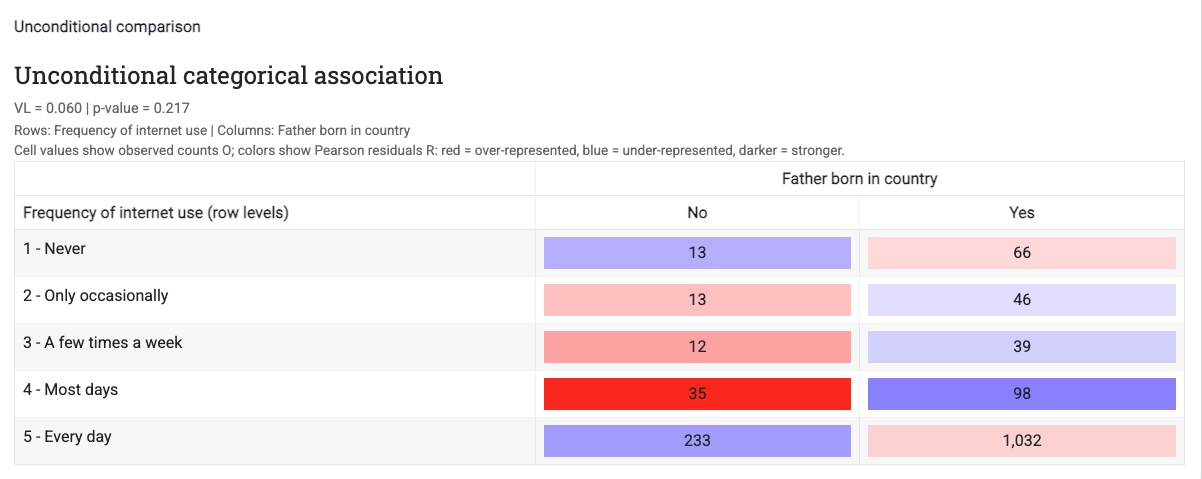
\includegraphics[width=\linewidth]{section3.3_unconditional_pairplot_netusoft_facntr.jpg}
\par\smallskip
\small Unconditional pair plot.
\end{minipage}
\hfill
\begin{minipage}{0.48\linewidth}
\centering
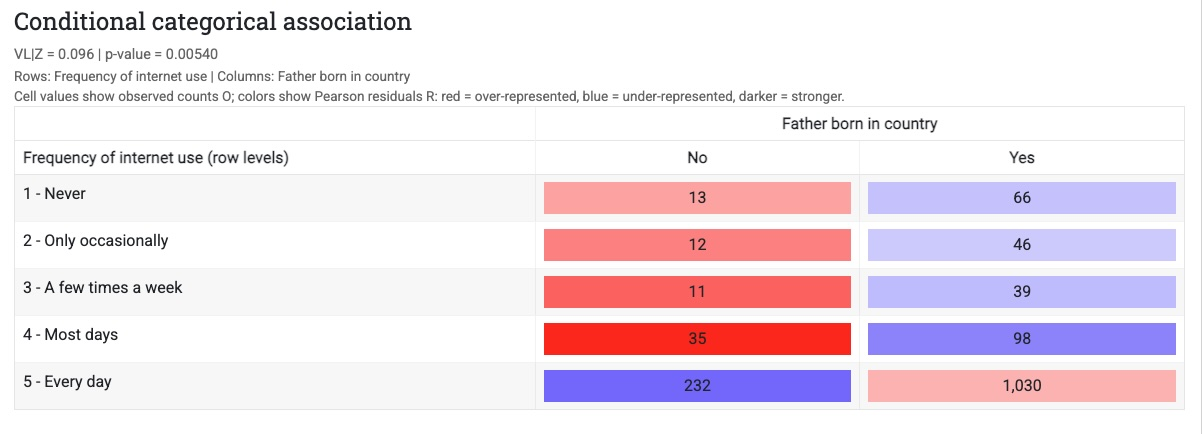
\includegraphics[width=\linewidth]{section3.3_conditional_pairplot_netusoft_facntr_agea.jpg}
\par\smallskip
\small Conditional pair plot with age of respondent (\code{agea}) as control.
\end{minipage}
\caption{\label{fig:catcatshots} Illustrative categorical--categorical pair
plots from the 2011 Belgian ESS for frequency of internet use
(\code{netusoft}) and father born in country (\code{facntr}). The cells print
observed counts, while colour encodes the Pearson residual relative to the
fitted null model. The conditional panel adjusts for age of respondent
(\code{agea}).}
\end{figure}

\section{Implementation details}
\label{sec:implementation}

The app is not merely a front-end around naive
repeated estimation. Several design choices in the implementation materially
improve responsiveness, especially for the categorical--categorical module.

First, the app builds a prepared problem object for each categorical pair. This
object stores the cleaned factor levels, the joint outcome mapping, the
control-design matrix, and grouped counts. The same prepared object is then
reused by the null and alternative models. This avoids repeated preprocessing
and ensures that both hypotheses are fit on exactly the same representation of
the data.

Second, repeated rows of the control-design matrix are collapsed into grouped
counts before evaluating the likelihood. If several observations share the same
coded control vector, their contributions are accumulated once and weighted by
their frequency. This does not change the model or the maximized likelihood, but
it reduces the number of rows over which the categorical likelihood must be
evaluated. The grouped likelihood is written explicitly in the appendix.

Third, the categorical models are estimated with \code{optim()} using an
analytic gradient rather than by finite-difference approximation. The
alternative model is warm-started from the null-model estimate by adding
zero-valued interaction parameters before optimization. This substantially
reduces the amount of work needed to move from the null to the alternative
model.

Fourth, the app caches pairwise results. Since users often revisit the same
variables while changing filters or switching between network and pair-plot
views, caching avoids refitting the same pairwise models unnecessarily.

The app also includes a specific solution for large categorical pair
plots. A full contingency table is displayed as long as the number of cells does
not exceed $49$. Beyond that threshold, the app selects a submatrix with at
most seven rows and seven columns. The selection score is the squared Pearson
residual
\begin{equation}
S_{ij} = R_{ij}^2
=
\frac{\left(O_{ij} - \widehat{E}^{(0)}_{ij}\right)^2}
     {\widehat{E}^{(0)}_{ij}},
\label{eq:score}
\end{equation}
which is the exact cellwise contribution to Pearson's chi-square statistic
$X^2 = \sum_{i,j} R_{ij}^2$. It is not a cellwise contribution to the
likelihood-ratio statistic $G^2$. However, under the null model and standard
regularity conditions, $X^2$ and $G^2$ are asymptotically equivalent: both
converge to the same $\chi^2$ limit and differ only by higher-order terms.
This score is therefore more suitable for display selection than cellwise
likelihood-ratio terms because $R_{ij}^2$ is symmetric in over- and
under-representation, remains informative for empty but unexpected cells, and
aligns directly with the colour scale shown in the pair plot. If
$m_r = \min(I,7)$ and $m_c = \min(J,7)$ denote the display limits, the app
solves
\begin{equation}
\max_{u,v,z}\sum_{i=1}^{I}\sum_{j=1}^{J} S_{ij} z_{ij}
\label{eq:subobjective}
\end{equation}
subject to
\begin{align}
\sum_{i=1}^{I} u_i &= m_r,
&
\sum_{j=1}^{J} v_j &= m_c,
\label{eq:subcons1}
\\
z_{ij} &\le u_i,
&
z_{ij} &\le v_j,
\label{eq:subcons2}
\\
z_{ij} &\ge u_i + v_j - 1.
\label{eq:subcons3}
\end{align}
Here $u_i$ and $v_j$ indicate selected rows and columns, while $z_{ij}$
indicates whether cell $(i,j)$ belongs to the displayed submatrix. The exact
optimization is carried out with \pkg{lpSolve} \citep{lpSolve} when available
and otherwise falls back to a heuristic based on the largest positive scores
$S_{ij}$. Because the display score and the cell value are both driven by
$R_{ij}$, the selected submatrix emphasizes precisely the standardized local
departures that the user ultimately sees. Additional details on the display
score and the retained-score coverage statistic are given in
Appendix~\ref{app:submatrix} (p.~\pageref{app:submatrix}).

Finally, the interface is designed to support comparison rather than only
inspection. When controls are selected, the network view can be switched
between conditional and unconditional structures, and the pair-plot section can
show the unconditional comparison below the conditional plot for the same pair.
This makes it easier to understand not only whether an association is retained,
but also how the local structure changes after adjustment.

\section{Illustrative analysis workflow}
\label{sec:example}

To illustrate the workflow, consider a Belgian extract of the European Social
Survey and suppose a user wants to identify the dependence structure linking
five variables: frequency of internet use (\code{netusoft}), self-rated health
(\code{health}), frequency of alcohol consumption (\code{alcfreq}), frequency
of social meetings (\code{sclmeet}), and vaccination status (\code{vacc19}).
The aim is not to test one pre-specified hypothesis, but to obtain an
interpretable overview of how these variables are related to one another within
a common association network.

\begin{figure}[H]
\centering
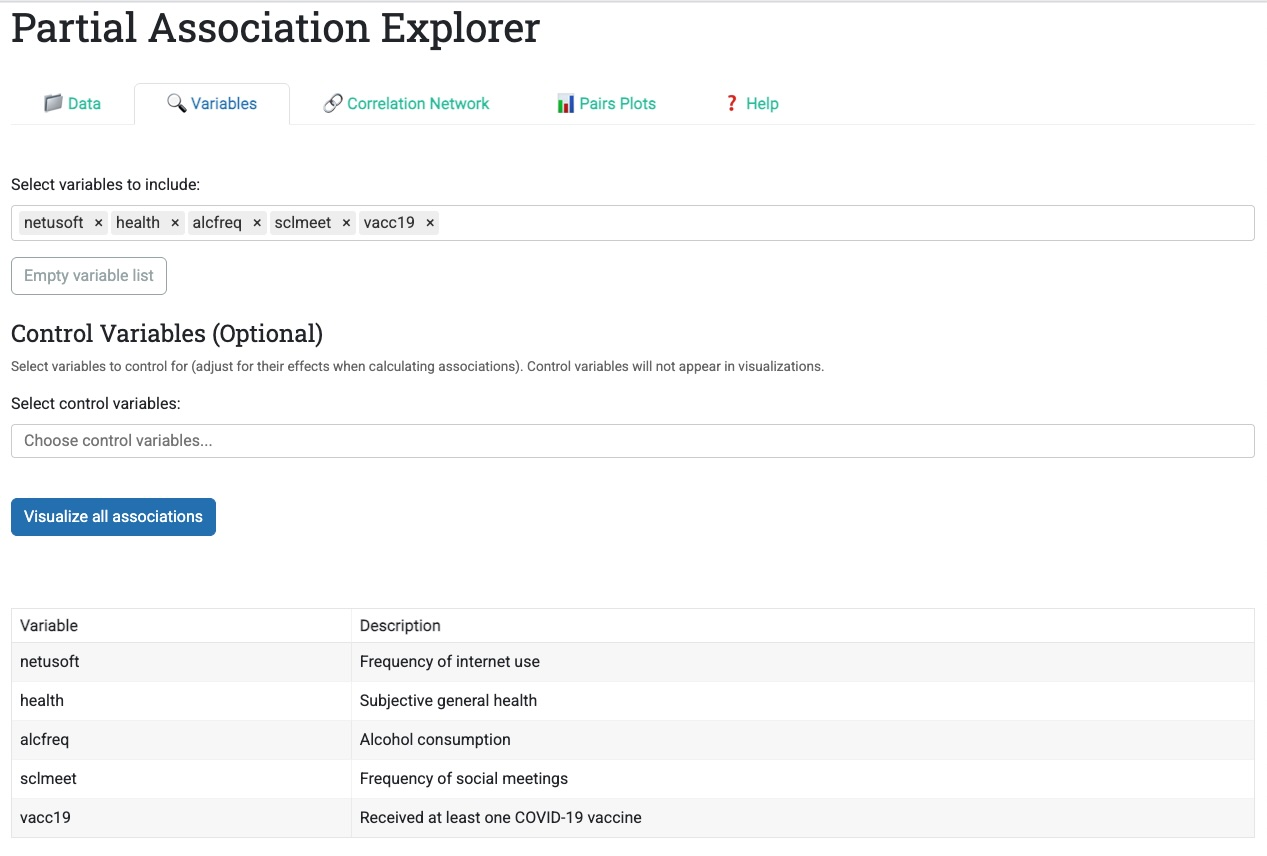
\includegraphics[width = 0.82\linewidth]{section5_variables_selection.jpg}

\medskip

\begin{minipage}{0.48\linewidth}
\centering
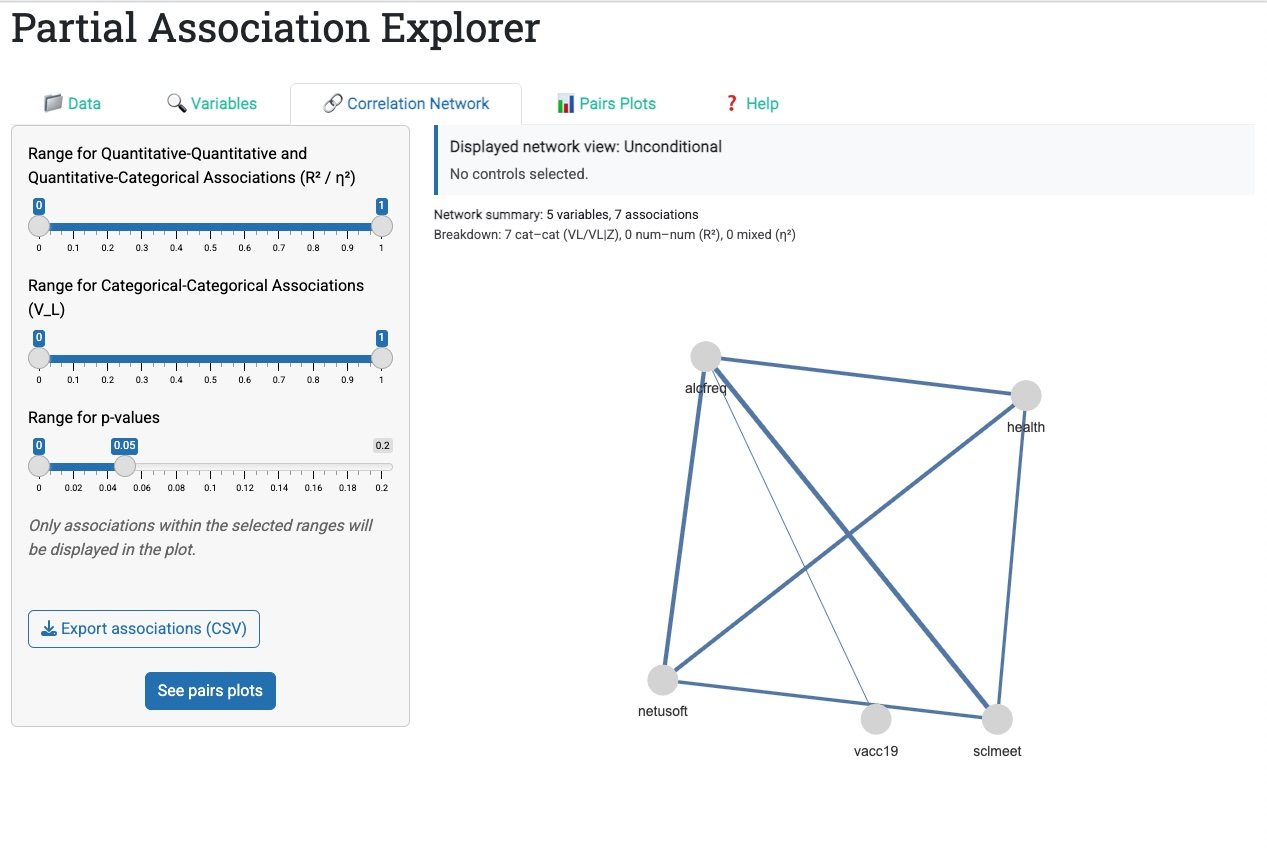
\includegraphics[width = \linewidth]{section5_unconditional_network.jpg}
\par\smallskip
\small (a) Unconditional association network.
\end{minipage}
\hfill
\begin{minipage}{0.48\linewidth}
\centering
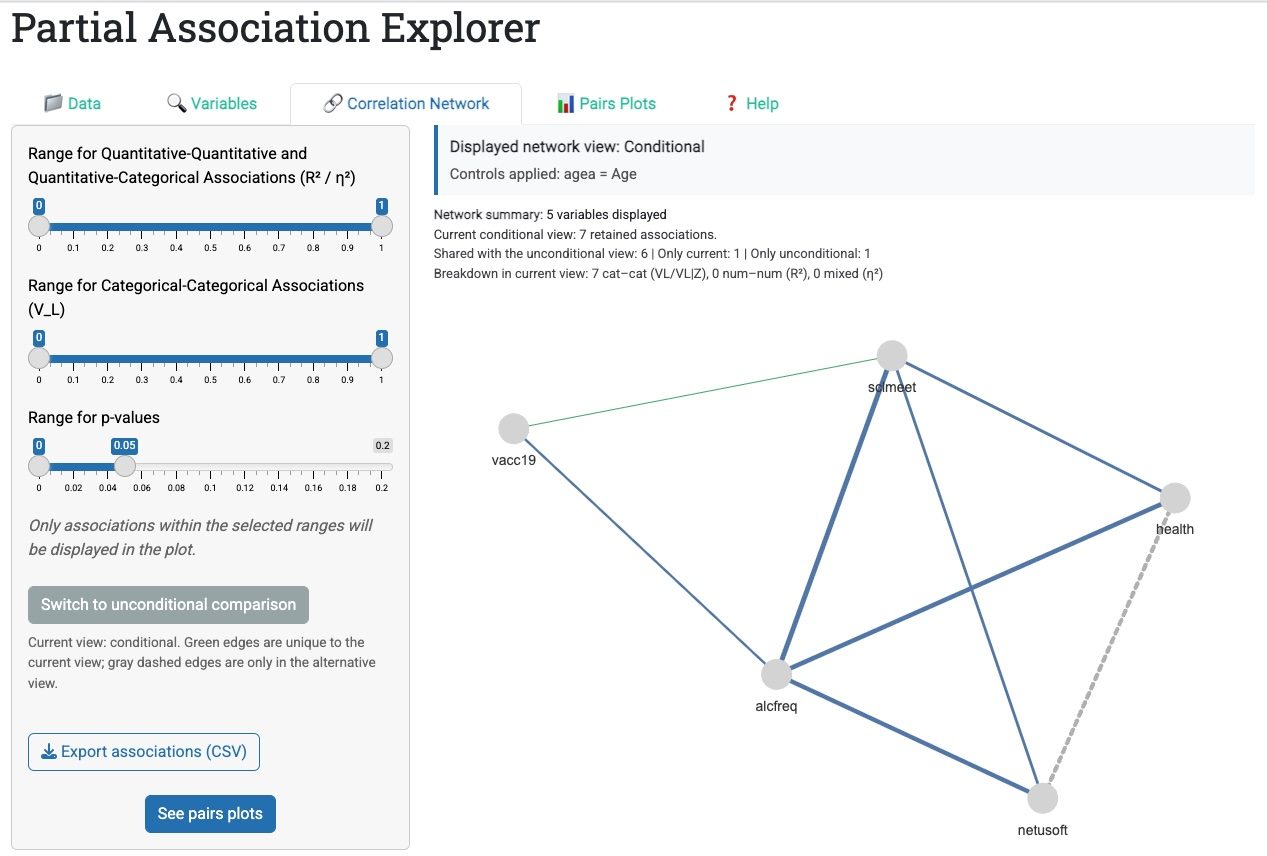
\includegraphics[width = \linewidth]{section5_conditional_network.jpg}
\par\smallskip
\small (b) Conditional association network with age of respondent (\code{agea}) as control.
\end{minipage}
\caption{\label{fig:networkexample} Illustrative workflow in \appname{}.
Top: selected analysis variables. Bottom-left: unconditional network.
Bottom-right: conditional network after controlling for age of respondent
(\code{agea}). The edge between self-rated health (\code{health}) and
frequency of internet use (\code{netusoft}) is retained without controls but
disappears after conditioning on age, whereas the edge between frequency of
social meetings (\code{sclmeet}) and vaccination status (\code{vacc19})
appears only in the conditional view.}
\end{figure}

The user first performs the analysis without controls and filters the network
by retaining only associations with $p$-values below 0.05. This unconditional
view already yields a compact map of the dependence structure. Several links
are visible, including an association between \code{health} and
\code{netusoft}. At first sight this suggests that respondents who use the
internet more frequently also tend to report better health. Figure
\ref{fig:networkexample} shows the resulting network, while the pair plot in
Figure~\ref{fig:healthinternet} clarifies the direction of the
relationship. Respondents who never use the internet are under-represented in
the \emph{very good} health category and over-represented in the \emph{fair}
and \emph{very bad} categories, whereas daily internet users show the reverse
pattern. Read as a whole, the table suggests a simple marginal association:
more frequent internet use is associated with better self-rated health.

This pattern is substantively plausible, but it is also a natural candidate for
confounding. The user may reasonably suspect that age plays an important role,
since age is often related both to internet use and to health, as well as to
other social behaviours recorded in the survey. In other words, age is a common
background variable that may shape the entire dependence structure rather than a
single pairwise association.

The user therefore adds age (\code{agea}) as a control and reruns the
analysis. The conditional network in Figure~\ref{fig:networkexample} reveals a
more surprising result than a simple global weakening. The total number of
retained edges remains similar, but the composition of the graph changes. The
edge between \code{health} and \code{netusoft}, clearly visible in the
unconditional analysis, disappears after conditioning on age. At the same time,
the edge between \code{sclmeet} and \code{vacc19}, which was not retained in
the unconditional view, now enters the network.

\begin{figure}[H]
\centering
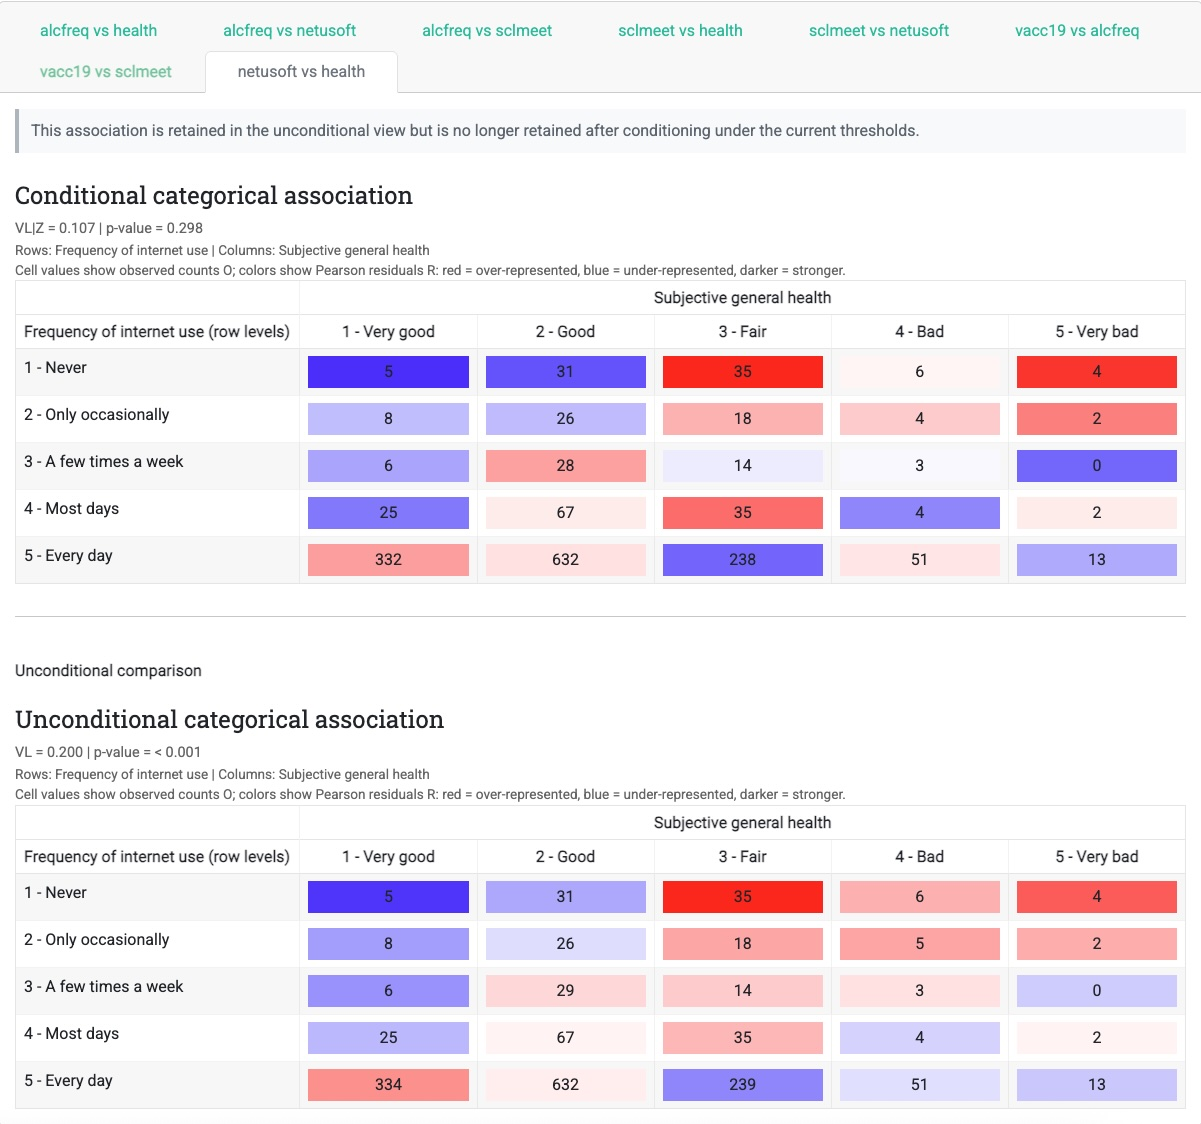
\includegraphics[width = 0.96\linewidth]{section5_pairplot_health_internet.jpg}
\caption{\label{fig:healthinternet} Conditional and unconditional pair plots
for frequency of internet use (\code{netusoft}) and self-rated health
(\code{health}) after adding age of respondent (\code{agea}) as control. The
pair is retained in the unconditional view but disappears from the conditional
network.}
\end{figure}

Figure~\ref{fig:healthinternet} explains the first change more formally.
Because both \code{health} and \code{netusoft} are categorical, the app reports
$V_L$ in the unconditional case and $V_{L\mid Z}$ in the conditional case.
Without controls, the association is moderate and statistically significant
($V_L = 0.200$, $p < 0.001$). After conditioning on age, it drops to
$V_{L\mid Z} = 0.107$ with $p = 0.298$, so the null hypothesis of conditional
independence is no longer rejected at the chosen threshold. Substantively, this
suggests that much of the original relationship was driven by age composition:
younger respondents tend to use the internet more often and also tend to report
better health, creating an apparent association between the two variables.

At the same time, conditioning on age reveals a second and more unexpected
result. The pair \code{sclmeet}--\code{vacc19} is not retained in the
unconditional analysis ($V_L = 0.085$, $p = 0.074$), so a user inspecting only
the marginal network would not identify it as relevant. After controlling for
age, however, the association becomes statistically significant and enters the
conditional graph ($V_{L\mid Z} = 0.105$, $p = 0.0078$). A plausible
interpretation is that age masks the relationship in the raw data: younger
respondents tend to report more frequent social meetings, whereas older
respondents are more likely to be vaccinated. These opposite age gradients
partly offset one another in the marginal table. Once comparisons are made
within age groups, a clearer pattern emerges in which respondents with more
frequent social contact are also more likely to be vaccinated. This second
change is illustrated by the pair-plot screenshot in
Figure~\ref{fig:sclmeetvacc}.

\begin{figure}[H]
\centering
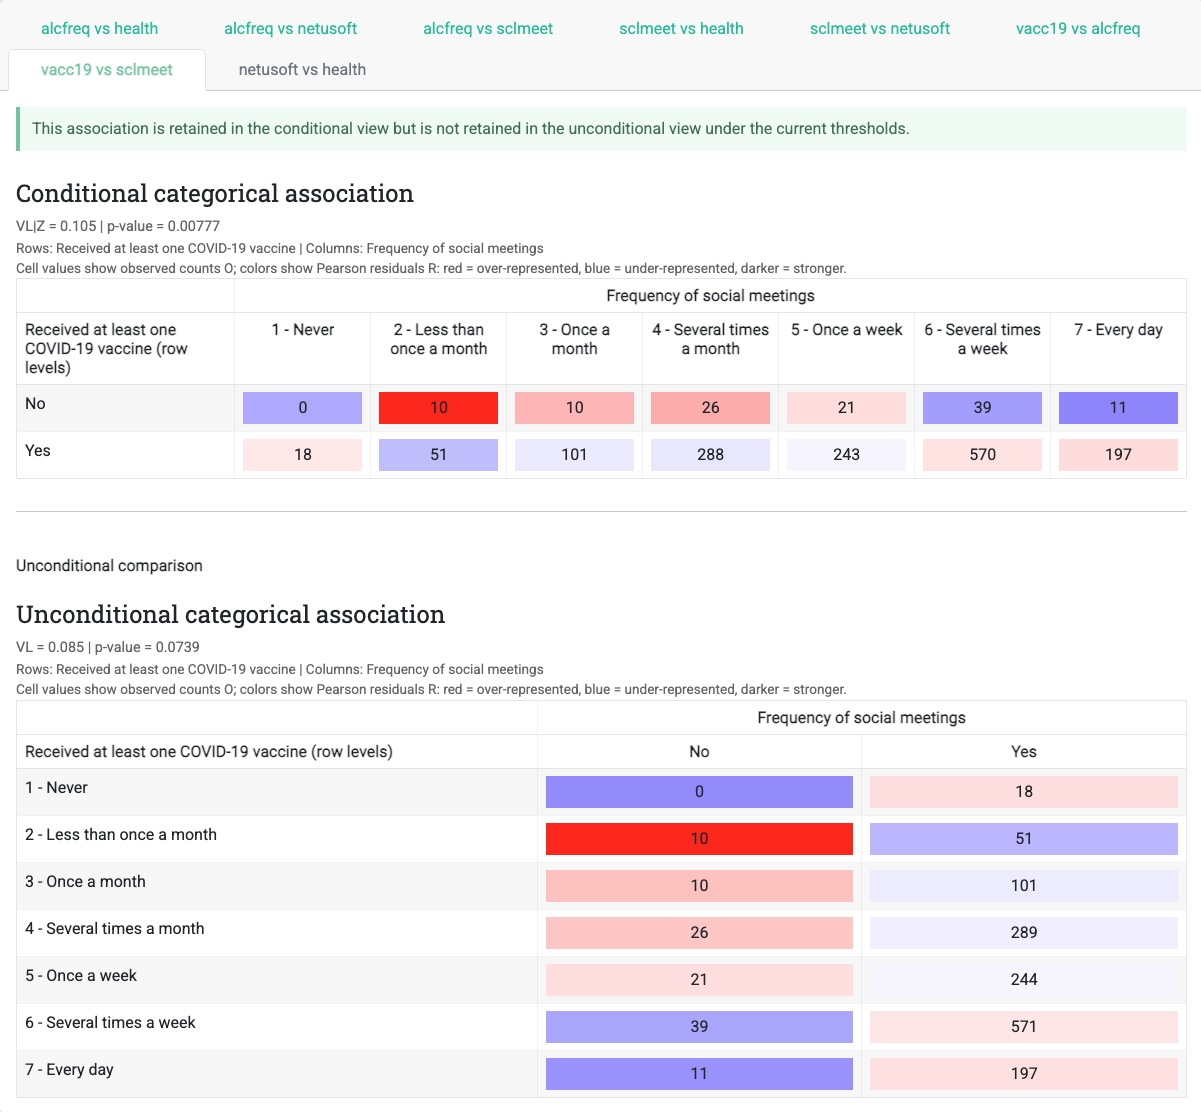
\includegraphics[width = 0.96\linewidth]{section5_pairplot_sclmeet_vacc19.jpg}
\caption{\label{fig:sclmeetvacc} Conditional and unconditional pair plots for
frequency of social meetings (\code{sclmeet}) and vaccination status
(\code{vacc19}) after adding age of respondent (\code{agea}) as control. The
association is not retained in the unconditional view but appears after
adjustment for age.}
\end{figure}

This example captures the intended use of \appname{}. A user begins by mapping
the unconditional dependence structure among a set of variables, then asks
whether a plausible background variable such as age may be shaping the observed
pattern. By introducing age as a control, the software turns a descriptive
network into a more informative analysis of confounding: one edge
(\code{netusoft}--\code{health}) disappears because it was largely compositional,
while another (\code{sclmeet}--\code{vacc19}) becomes visible only after
adjustment.

\section{Related software}
\label{sec:related}

The closest software comparison is the earlier \pkg{AssociationExplorer}
\citep{SoeteweyHeuchenneClaesDescampe2026}, from which \appname{} inherits the
basic idea of exploring associations through a network and pairwise plots in a
\pkg{shiny} interface. The main extensions are the introduction of control
variables, the computation of formal tests for every selected pair, the
likelihood-based treatment of categorical--categorical associations, and the
expanded local diagnostics.

Another relevant comparison is \emph{Sirius}, a Python and Django application
for exploratory visualization of mixed data based on mutual information
networks and backbone sparsification \citep{AdamsEtAl2021}. Sirius shares with
\appname{} the objective of helping users navigate heterogeneous dependence
structures visually. The two tools nevertheless emphasize different tasks.
Sirius uses a common information-theoretic score across mixed feature pairs and
focuses on network-level exploration, whereas \appname{} adopts
pair-type-specific association measures, attaches a formal test to every edge,
and gives users an explicit conditional workflow in which chosen control
variables can remove spurious associations or reveal masked ones. Its local
diagnostics are likewise tied directly to the statistical model used for each
pair type.

More generally, analysts can assemble pieces of a similar workflow from base
\proglang{R} and general-purpose packages. Numerical correlations can be
computed with standard correlation functions; numerical--categorical
relationships can be assessed through linear models or ANOVA; and
contingency-table analyses can be carried out with standard categorical-data
tools. Some mixed-data packages instead focus on dimension reduction or
multivariate description rather than pairwise conditional interpretation.
However, assembling a workflow comparable to \appname{} usually requires moving
manually between different model objects, plotting systems, and data
representations. In contrast, \appname{} offers one interface in which all pair
types are treated jointly, the network is filtered using a common visual
grammar, and optional controls can be applied consistently across the full set
of pairs.

The app should therefore be understood less as a competitor
to any single-purpose package and more as a unifying exploratory layer that
connects several standard statistical ideas within one workflow.

\section{Discussion}
\label{sec:discussion}

\appname{} contributes in five main ways. First, it unifies global association
measures for all common pair types in a single interface. Second, it makes
conditional association analysis accessible without requiring users to write
regression, ANOVA, or multinomial likelihood code by hand. Third, it combines
effect-size filtering with formal significance tests so that users can tune the
network with strength and $p$-value sliders rather than relying on one
threshold alone. Fourth, it makes the unconditional--conditional comparison
explicit, allowing users to detect spurious associations that disappear after
adjustment and hidden associations that emerge only conditionally. Fifth, it
connects global network edges to local diagnostics,
which is especially important for categorical data where a single global
statistic may be driven by a limited number of over- or under-represented
cells.

The software is not intended to establish causal effects. Conditional
associations depend on the selected controls and on the adequacy of the working
models. Sparse categorical tables, rare categories, separation-like behaviour
in multinomial fitting, and misspecified control effects may affect the
reliability of both global and local summaries. The app should therefore be
understood as a transparent exploratory layer that helps users decide where
more formal modelling is warranted.

A more specific limitation concerns how variable types are detected.
In the app, a variable is treated as numerical when
\code{is.numeric()} returns true in \proglang{R}; otherwise it is handled as
categorical. This rule is transparent and easy to reproduce, but it is tied to
storage class rather than to measurement meaning. Ordered factors, Likert-type
items, and other ordinal variables imported as factors therefore enter the
categorical branch by default. When such variables have many ordered levels,
this can enlarge contingency tables, reduce stability in sparse cells, and send
the analysis toward likelihood-based categorical measures even when a user might
prefer a numerical approximation.

A related limitation is that the three global measures are bounded on the same
$[0,1]$ scale but are not substantively identical. $R^2$ and $\eta^2$ are
variance-explained quantities tied to linear-model decompositions, whereas
$V_L$ is a monotone transformation of a per-observation likelihood improvement.
As a result, a common slider threshold remains an exploratory convenience rather
than a theoretically exact cross-type standard. The issue becomes sharper when
ordinal variables could plausibly be encoded either way: the same five-category
pair might in principle yield a moderate $V_L$ when treated as categorical but
a much smaller $R^2$ if recoded numerically, because the two representations
summarize different model families and different notions of association.

These limitations suggest several extensions. One is to let users override the
automatically detected type more explicitly and to add dedicated ordinal
handling, for example through polychoric or polyserial alternatives, ordinal
regression-based measures, or side-by-side sensitivity analyses under different
codings. Another is to provide a suggestion layer based on variable labels,
value patterns, or external metadata, potentially assisted by language models,
to flag large ordered categorical variables that may deserve special treatment.

\section*{Computational details}

The application is implemented in \proglang{R} and distributed through a public
GitHub repository at
\url{https://github.com/Thadhaeg/Partial-association-explorer}. The user
interface relies primarily on \pkg{shiny} \citep{Shiny}, \pkg{bslib}
\citep{bslib}, \pkg{shinyjs} \citep{shinyjs}, and \pkg{visNetwork}
\citep{VisNetwork}. Tabular displays rely on \pkg{reactable}
\citep{reactable}. Data import and preprocessing use \pkg{readxl}
\citep{readxl} and \pkg{janitor} \citep{janitor}. The network backend uses
\pkg{tidygraph} \citep{tidygraph}. When available, exact large-table submatrix
selection is performed with \pkg{lpSolve} \citep{lpSolve}.

The screenshots included in this article were generated from the app as of
2026-07-10. The code is available through the public GitHub repository and the
manuscript can be complemented, before submission, with a fully reproducible
analysis script if required by the review process.

\begin{thebibliography}{17}

\bibitem[Agresti(2013)]{Agresti2013}
Agresti A (2013).
\newblock \emph{Categorical Data Analysis}.
\newblock 3rd edition. Wiley, Hoboken.

\bibitem[Adams et~al.(2021)]{AdamsEtAl2021}
Adams JL, Deluca TF, Danforth CM, Dodds PS, Zheng Y, Anastasakis K, Choi B,
Min A, Bessey MM (2021).
\newblock ``Sirius: A Mutual Information Tool for Exploratory Visualization of
Mixed Data.''
\newblock arXiv:2106.05260.
\newblock \url{https://arxiv.org/abs/2106.05260}.

\bibitem[Almende BV and Contributors and Thieurmel(2025)]{VisNetwork}
Almende BV and Contributors, Thieurmel B (2025).
\newblock \emph{\pkg{visNetwork}: Network Visualization Using vis.js Library}.
\newblock \proglang{R} package version 2.1.4,
\url{https://CRAN.R-project.org/package=visNetwork}.
\newblock \doi{10.32614/CRAN.package.visNetwork}.

\bibitem[Attali(2021)]{shinyjs}
Attali D (2021).
\newblock \emph{\pkg{shinyjs}: Easily Improve the User Experience of Your Shiny Apps in Seconds}.
\newblock \proglang{R} package version 2.1.0,
\url{https://CRAN.R-project.org/package=shinyjs}.
\newblock \doi{10.32614/CRAN.package.shinyjs}.

\bibitem[Berkelaar(2024)]{lpSolve}
Berkelaar M (2024).
\newblock \emph{\pkg{lpSolve}: Interface to Lp\_solve v. 5.5 to Solve Linear/Integer Programs}.
\newblock \proglang{R} package version 5.6.23,
\url{https://CRAN.R-project.org/package=lpSolve}.
\newblock \doi{10.32614/CRAN.package.lpSolve}.

\bibitem[Chang et~al.(2026)]{Shiny}
Chang W, Cheng J, Allaire J, Sievert C, Schloerke B, Xie Y, Allen J,
McPherson J, Dipert A, Borges B (2026).
\newblock \emph{\pkg{shiny}: Web Application Framework for \proglang{R}}.
\newblock \proglang{R} package,
\url{https://CRAN.R-project.org/package=shiny}.

\bibitem[Cox and Snell(1989)]{CoxSnell1989}
Cox DR, Snell EJ (1989).
\newblock \emph{Analysis of Binary Data}.
\newblock 2nd edition. Chapman and Hall, London.

\bibitem[Firke(2024)]{janitor}
Firke S (2024).
\newblock \emph{\pkg{janitor}: Simple Tools for Examining and Cleaning Dirty Data}.
\newblock \proglang{R} package version 2.2.1,
\url{https://CRAN.R-project.org/package=janitor}.
\newblock \doi{10.32614/CRAN.package.janitor}.

\bibitem[Hamdan and Tsokos(1971)]{HamdanTsokos1971}
Hamdan MA, Tsokos CP (1971).
\newblock ``An Information Measure of Association in Contingency Tables.''
\newblock \emph{Information and Control}, \textbf{19}(2), 174--179.
\newblock \doi{10.1016/S0019-9958(71)90799-6}.

\bibitem[Lin(2023)]{reactable}
Lin G (2023).
\newblock \emph{\pkg{reactable}: Interactive Data Tables for \proglang{R}}.
\newblock \proglang{R} package version 0.4.4,
\url{https://CRAN.R-project.org/package=reactable}.
\newblock \doi{10.32614/CRAN.package.reactable}.

\bibitem[Linfoot(1957)]{Linfoot1957}
Linfoot EH (1957).
\newblock ``An Informational Measure of Correlation.''
\newblock \emph{Information and Control}, \textbf{1}(1), 85--89.
\newblock \doi{10.1016/S0019-9958(57)90116-X}.

\bibitem[McFadden(1974)]{McFadden1974}
McFadden D (1974).
\newblock ``Conditional Logit Analysis of Qualitative Choice Behavior.''
\newblock In P Zarembka (ed.), \emph{Frontiers in Econometrics}, pp. 105--142.
Academic Press, New York.

\bibitem[Nagelkerke(1991)]{Nagelkerke1991}
Nagelkerke NJD (1991).
\newblock ``A Note on a General Definition of the Coefficient of Determination.''
\newblock \emph{Biometrika}, \textbf{78}(3), 691--692.
\newblock \doi{10.1093/biomet/78.3.691}.

\bibitem[Nelder and Wedderburn(1972)]{NelderWedderburn1972}
Nelder JA, Wedderburn RWM (1972).
\newblock ``Generalized Linear Models.''
\newblock \emph{Journal of the Royal Statistical Society. Series A},
\textbf{135}(3), 370--384.

\bibitem[Pedersen(2024)]{tidygraph}
Pedersen TL (2024).
\newblock \emph{\pkg{tidygraph}: A Tidy API for Graph Manipulation}.
\newblock \proglang{R} package version 1.3.1,
\url{https://CRAN.R-project.org/package=tidygraph}.
\newblock \doi{10.32614/CRAN.package.tidygraph}.

\bibitem[{\proglang{R} Core Team}(2026)]{R}
{\proglang{R} Core Team} (2026).
\newblock \emph{\proglang{R}: A Language and Environment for Statistical Computing}.
\newblock \proglang{R} Foundation for Statistical Computing, Vienna, Austria.
\newblock \url{https://www.R-project.org/}.

\bibitem[Sievert et~al.(2025)]{bslib}
Sievert C, Cheng J, Aden-Buie G (2025).
\newblock \emph{\pkg{bslib}: Custom Bootstrap Sass Themes for \pkg{shiny} and \pkg{rmarkdown}}.
\newblock \proglang{R} package version 0.9.0,
\url{https://CRAN.R-project.org/package=bslib}.
\newblock \doi{10.32614/CRAN.package.bslib}.

\bibitem[Soetewey et~al.(2026)]{SoeteweyHeuchenneClaesDescampe2026}
Soetewey A, Heuchenne C, Claes A, Descampe A (2026).
\newblock \emph{\pkg{AssociationExplorer}: A User-Friendly \pkg{shiny} Application for Exploring Associations and Visual Patterns}.
\newblock \emph{SoftwareX}, \textbf{33}, 102483.
\newblock \doi{10.1016/j.softx.2025.102483}.

\bibitem[Wickham and Bryan(2026)]{readxl}
Wickham H, Bryan J (2026).
\newblock \emph{\pkg{readxl}: Read Excel Files}.
\newblock \proglang{R} package version 1.5.0,
\url{https://CRAN.R-project.org/package=readxl}.
\newblock \doi{10.32614/CRAN.package.readxl}.

\end{thebibliography}

\newpage

\begin{appendix}

\section{Supplementary computational details for numerical--numerical associations}
\label{app:numnum}

This appendix records the explicit quantities computed by the app for
numerical--numerical pairs in the unconditional and conditional cases.

\subsection{Unconditional case}

Given numerical variables $X$ and $Y$ observed on $n$ units, the app first
computes Pearson's correlation
\begin{equation}
r_{XY}
=
\frac{
\sum_{t=1}^{n}(X_t - \bar{X})(Y_t - \bar{Y})
}{
\sqrt{\sum_{t=1}^{n}(X_t - \bar{X})^2}
\sqrt{\sum_{t=1}^{n}(Y_t - \bar{Y})^2}
}.
\label{eq:app-pearson}
\end{equation}
The network is filtered on the squared quantity
\begin{equation}
R^2_{XY} = r_{XY}^2.
\label{eq:app-r2}
\end{equation}
For inference, the null hypothesis $H_0: r_{XY} = 0$ is tested with
\begin{equation}
T
=
r_{XY}\sqrt{\frac{n-2}{1-r_{XY}^2}},
\label{eq:app-t-pearson}
\end{equation}
which is equivalent to the one-degree-of-freedom $F$ statistic
\begin{equation}
F = T^2 \sim F_{1,n-2}.
\label{eq:app-f-pearson}
\end{equation}
The app reports the corresponding two-sided $p$-value through this equivalent
$F$ representation.

\subsection{Conditional case}

With controls $Z = (Z_1, \dots, Z_q)$, the app computes the partial
correlation through residualization. It first fits linear regressions
\begin{equation}
X_t = a_X + \sum_{k=1}^{q} b_{Xk} Z_{kt} + u^X_t,
\qquad
Y_t = a_Y + \sum_{k=1}^{q} b_{Yk} Z_{kt} + u^Y_t,
\label{eq:app-resid-models}
\end{equation}
and then forms the residuals
\begin{equation}
\tilde{X}_t = \hat{u}^X_t = X_t - \widehat{\mathbb{E}}(X_t \mid Z_t),
\qquad
\tilde{Y}_t = \hat{u}^Y_t = Y_t - \widehat{\mathbb{E}}(Y_t \mid Z_t).
\label{eq:app-resids}
\end{equation}
The conditional association measure is the squared partial correlation
\begin{equation}
r_{XY\mid Z} = \mathrm{cor}(\tilde{X}, \tilde{Y}),
\qquad
R^2_{XY\mid Z} = r_{XY\mid Z}^2.
\label{eq:app-partial-r}
\end{equation}
To test $H_0: r_{XY\mid Z} = 0$, the app uses
\begin{equation}
T_{\mathrm{cond}}
=
r_{XY\mid Z}\sqrt{\frac{n-q-2}{1-r_{XY\mid Z}^2}},
\label{eq:app-t-partial}
\end{equation}
or equivalently
\begin{equation}
F_{\mathrm{cond}} = T_{\mathrm{cond}}^2 \sim F_{1,n-q-2}.
\label{eq:app-f-partial}
\end{equation}
The implementation counts only controls with non-zero variation in the
effective value of $q$.

\subsection{Pair plots}

Without controls, the pair plot is the raw scatter of $(X_t, Y_t)$ with a
fitted linear trend. With controls, it is the added-variable plot formed by
the residual pairs $(\tilde{X}_t, \tilde{Y}_t)$. In both cases the plot gives
the local pattern behind the global $R^2$ measure, while the sign of the slope
reflects the sign of the corresponding correlation coefficient.

\section{Supplementary computational details for numerical--categorical associations}
\label{app:numcat}

Let $Y$ be numerical and let $X$ be categorical with levels
$1, \dots, J$.

\subsection{Unconditional case}

The app uses the ANOVA decomposition. Writing $\bar{Y}$ for the overall mean,
$\bar{Y}_j$ for the mean in group $j$, and $n_j$ for the group size, it
computes
\begin{equation}
\mathrm{SST} = \sum_{t=1}^{n}(Y_t - \bar{Y})^2,
\qquad
\mathrm{SSB} = \sum_{j=1}^{J} n_j (\bar{Y}_j - \bar{Y})^2.
\label{eq:app-sst-ssb}
\end{equation}
The global association measure is
\begin{equation}
\eta^2 = \frac{\mathrm{SSB}}{\mathrm{SST}}.
\label{eq:app-eta2}
\end{equation}
The null hypothesis of equal group means is tested with the ANOVA statistic
\begin{equation}
F
=
\frac{\mathrm{SSB}/(J-1)}{\mathrm{SSW}/(n-J)},
\qquad
\mathrm{SSW} = \sum_{j=1}^{J}\sum_{t:X_t=j}(Y_t - \bar{Y}_j)^2,
\label{eq:app-anova-f}
\end{equation}
which is compared to an $F_{J-1,n-J}$ distribution.

\subsection{Conditional case}

With controls $Z = (Z_1, \dots, Z_q)$, the app uses an ANCOVA/extra-sum-of-
squares construction. The full model is
\begin{equation}
Y_t
=
\alpha
+ \sum_{j=2}^{J} \beta_j 1\{X_t = j\}
+ \sum_{k=1}^{q} \gamma_k Z_{kt}
+ \varepsilon_t,
\label{eq:app-full-ancova}
\end{equation}
whereas the reduced model omits the group indicators:
\begin{equation}
Y_t
=
\alpha'
+ \sum_{k=1}^{q} \gamma'_k Z_{kt}
+ \varepsilon'_t.
\label{eq:app-red-ancova}
\end{equation}
Here $\alpha$ is the intercept of the full ANCOVA model, $\beta_j$ is the
effect of category $j$ of $X$ relative to the reference category, and
$\gamma_k$ is the slope associated with control $Z_k$. The primed quantities
in the reduced model play the same roles after the categorical predictor has
been removed.
Let $\mathrm{RSS}_{\mathrm{full}}$ and $\mathrm{RSS}_{\mathrm{red}}$ denote
their residual sums of squares. The extra sum of squares attributable to $X$
given $Z$ is
\begin{equation}
\mathrm{SS}(X \mid Z)
=
\mathrm{RSS}_{\mathrm{red}} - \mathrm{RSS}_{\mathrm{full}},
\label{eq:app-ssxz}
\end{equation}
and the app computes
\begin{equation}
\eta^2_{X\mid Z}
=
\frac{\mathrm{SS}(X \mid Z)}
{\mathrm{SS}(X \mid Z) + \mathrm{RSS}_{\mathrm{full}}}.
\label{eq:app-partial-eta2}
\end{equation}
The corresponding test statistic is
\begin{equation}
F_{\mathrm{cond}}
=
\frac{[\mathrm{RSS}_{\mathrm{red}} - \mathrm{RSS}_{\mathrm{full}}]/(J-1)}
{\mathrm{RSS}_{\mathrm{full}}/\mathrm{df}_2},
\label{eq:app-ancova-f}
\end{equation}
where $\mathrm{df}_2$ is the residual degrees of freedom of the full model.
This is compared to an $F_{J-1,\mathrm{df}_2}$ distribution.

\subsection{Pair plots}

Without controls, the pair plot displays the raw group means
\begin{equation}
\bar{Y}_j = \frac{1}{n_j}\sum_{t:X_t=j} Y_t.
\label{eq:app-group-means}
\end{equation}
With controls, the app first residualizes the numerical outcome by fitting
\begin{equation}
Y_t = a + \sum_{k=1}^{q} \delta_k Z_{kt} + u_t
\label{eq:app-y-on-z}
\end{equation}
and computing
\begin{equation}
\tilde{Y}_t = \hat{u}_t = Y_t - \widehat{\mathbb{E}}(Y_t \mid Z_t).
\label{eq:app-y-resid}
\end{equation}
It then displays the residualized group means
\begin{equation}
\bar{\tilde{Y}}_j
=
\frac{1}{n_j}\sum_{t:X_t=j}\tilde{Y}_t.
\label{eq:app-resid-means}
\end{equation}
Here $a$ is the intercept of the residualization regression, and each
$\delta_k$ is the slope attached to control $Z_k$. Thus $\delta_k$ measures the
linear contribution of the $k$th control to the numerical outcome before group
means are recomputed from the residuals.
These bars show the remaining group differences after the linear dependence of
$Y$ on the controls has been removed.

\section{Supplementary computational details for categorical--categorical associations}
\label{app:catcat}

The categorical--categorical module is based on a joint multinomial model for
$W = (X, Y)$, treated as a single categorical outcome with $K = IJ$ possible
cells.

\subsection{Unconditional case}

Under the null model of independence, the linear predictor for cell $(i,j)$ is
\begin{equation}
\eta^{(0)}_{ij} = \alpha_i + \beta_j,
\label{eq:app-eta0}
\end{equation}
whereas the alternative model adds interaction terms
\begin{equation}
\eta^{(1)}_{ij} = \alpha_i + \beta_j + \gamma_{ij}.
\label{eq:app-eta1}
\end{equation}
Here $\alpha_i$ is the baseline effect associated with level $i$ of $X$,
$\beta_j$ is the baseline effect associated with level $j$ of $Y$, and
$\gamma_{ij}$ is the cell-specific interaction that measures the departure from
independence for combination $(i,j)$.
With first row and first column taken as references, the constraints are
\begin{equation}
\alpha_1 = 0,
\qquad
\beta_1 = 0,
\qquad
\gamma_{1j} = \gamma_{i1} = 0.
\label{eq:app-catcat-constraints}
\end{equation}
The implied probabilities are
\begin{equation}
\pi^{(m)}_{ij}
=
\frac{\exp(\eta^{(m)}_{ij})}
{\sum_{r=1}^{I}\sum_{s=1}^{J}\exp(\eta^{(m)}_{rs})},
\qquad m \in \{0,1\},
\label{eq:app-pi-uncond}
\end{equation}
and the observation-level log-likelihood is
\begin{equation}
\ell_m(\theta)
=
\sum_{t=1}^{n}\log \pi^{(m)}_{X_tY_t}(\theta).
\label{eq:app-loglik-uncond}
\end{equation}
The likelihood-ratio statistic is
\begin{equation}
G^2 = 2(\ell_1 - \ell_0),
\label{eq:app-g2-uncond}
\end{equation}
and the corresponding bounded association measure is
\begin{equation}
V_L = \sqrt{1 - \exp(-G^2/n)}.
\label{eq:app-vl-uncond}
\end{equation}
Under regularity conditions, the inference step compares $G^2$ to a
$\chi^2_{(I-1)(J-1)}$ distribution.

\subsection{Conditional case}

Let $Z = (Z_1, \dots, Z_q)$ denote the controls after model-matrix coding. The
null model of conditional independence is
\begin{equation}
\eta^{(0)}_{ij}(z)
=
\alpha_i + \beta_j
+ \sum_{k=1}^{q} \lambda_{ik} z_k
+ \sum_{k=1}^{q} \kappa_{jk} z_k,
\label{eq:app-eta0-cond}
\end{equation}
and the alternative adds cell interactions:
\begin{equation}
\eta^{(1)}_{ij}(z)
=
\alpha_i + \beta_j
+ \sum_{k=1}^{q} \lambda_{ik} z_k
+ \sum_{k=1}^{q} \kappa_{jk} z_k
+ \gamma_{ij}.
\label{eq:app-eta1-cond}
\end{equation}
In this conditional specification, $\alpha_i$ and $\beta_j$ remain the
baseline effects for categories of $X$ and $Y$. The coefficient
$\lambda_{ik}$ gives the contribution of control $Z_k$ to the logit component
associated with row category $i$, whereas $\kappa_{jk}$ gives the analogous
contribution for column category $j$. The interaction parameter $\gamma_{ij}$
again measures the residual cell-specific association once these main and
control effects have been taken into account.
The same reference-category structure is used, now together with
\begin{equation}
\lambda_{1k} = 0,
\qquad
\kappa_{1k} = 0
\qquad \text{for all } k.
\label{eq:app-cond-constraints}
\end{equation}
The conditional probabilities are
\begin{equation}
\pi^{(m)}_{ij}(z)
=
\frac{\exp(\eta^{(m)}_{ij}(z))}
{\sum_{r=1}^{I}\sum_{s=1}^{J}\exp(\eta^{(m)}_{rs}(z))},
\qquad m \in \{0,1\}.
\label{eq:app-pi-cond}
\end{equation}

To keep the main text readable, the theoretical definitions in
Equations~\eqref{eq:loglik} and \eqref{eq:e0} are written observation by
observation, indexed by $t$. In this appendix, the notation changes because
the app groups observations that share the same coded control vector. The
statistical definition is unchanged: only the bookkeeping differs, so repeated
terms are replaced by counts.

The implementation evaluates the conditional categorical likelihood on
grouped control-design rows rather than observation by observation. Let
$z^{(g)}$, $g = 1, \dots, G$, denote the distinct control-design rows after
model-matrix coding, and let $N_{gij}$ be the number of observations belonging
to cell $(i,j)$ within control group $g$. Then the grouped conditional
log-likelihood is
\begin{equation}
\ell_m(\theta) =
\sum_{g=1}^{G}\sum_{i=1}^{I}\sum_{j=1}^{J}
N_{gij}\log \pi^{(m)}_{ij}(z^{(g)}; \theta),
\qquad m \in \{0,1\}.
\label{eq:grouploglik}
\end{equation}
This is algebraically equivalent to the observation-level conditional
log-likelihood, but it is much faster to evaluate whenever many observations
share the same coded control vector.

The conditional likelihood-ratio statistic is
\begin{equation}
G^2_{\mid Z} = 2(\ell_1 - \ell_0),
\label{eq:app-g2-cond}
\end{equation}
and the conditional association measure is
\begin{equation}
V_{L\mid Z} = \sqrt{1 - \exp(-G^2_{\mid Z}/n)}.
\label{eq:app-vlz-cond}
\end{equation}
The same $(I-1)(J-1)$ degrees of freedom apply to the likelihood-ratio test
because the difference between the null and alternative models is exactly the
interaction block.

\subsection{Local diagnostics and pair plots}

Let $O_{ij}$ denote the observed cell count
\begin{equation}
O_{ij} = \sum_{t=1}^{n} 1\{X_t = i, Y_t = j\}.
\label{eq:app-oij}
\end{equation}
For both the unconditional and conditional modules, the expected count used by
the app is defined from the fitted null probabilities as
\begin{equation}
\widehat{E}^{(0)}_{ij}
=
\sum_{t=1}^{n}\Pr(X=i,Y=j \mid Z_t; \widehat{\theta}_0)
=
\sum_{t=1}^{n}\pi^{(0)}_{ij}(Z_t; \widehat{\theta}_0).
\label{eq:app-e0-generic}
\end{equation}
In the unconditional case, there are no controls and the fitted probability is
constant across observations, so this reduces to
\begin{equation}
\widehat{E}^{(0)}_{ij} = n \pi^{(0)}_{ij}(\widehat{\theta}_0).
\label{eq:app-e0-uncond}
\end{equation}
In the conditional case, the implementation groups identical control-design
rows. If $z^{(g)}$, $g = 1, \dots, G$, denotes a distinct coded control vector
and $n_g = \sum_{i,j} N_{gij}$ its frequency, then the same quantity can be
written as
\begin{equation}
\widehat{E}^{(0)}_{ij}
=
\sum_{g=1}^{G} n_g \pi^{(0)}_{ij}(z^{(g)}; \widehat{\theta}_0).
\label{eq:e0group}
\end{equation}

The pair plots are built from the observed-minus-expected deviation
\begin{equation}
D_{ij} = O_{ij} - \widehat{E}^{(0)}_{ij}
\label{eq:app-dij}
\end{equation}
and the Pearson residual
\begin{equation}
R_{ij}
=
\frac{O_{ij} - \widehat{E}^{(0)}_{ij}}
     {\sqrt{\widehat{E}^{(0)}_{ij}}}.
\label{eq:app-rij}
\end{equation}
The squared Pearson residual is the exact cellwise contribution to Pearson's
chi-square statistic:
\begin{equation}
X^2
=
\sum_{i=1}^{I}\sum_{j=1}^{J} R_{ij}^2
=
\sum_{i=1}^{I}\sum_{j=1}^{J}
\frac{\left(O_{ij} - \widehat{E}^{(0)}_{ij}\right)^2}
     {\widehat{E}^{(0)}_{ij}}.
\label{eq:app-x2}
\end{equation}
Thus $R_{ij}^2$, not $R_{ij}$ itself, is the relevant cellwise contribution.
This is not the same as a cellwise contribution to the likelihood-ratio
statistic $G^2$, whose multinomial decomposition involves terms of the form
$2\,O_{ij}\log(O_{ij}/\widehat{E}^{(0)}_{ij})$. In finite samples, $X^2$ and $G^2$ are
generally different. Under the null model and standard regularity conditions,
however, they are asymptotically equivalent in the sense that both converge to
the same $\chi^2$ limit and differ only by higher-order terms from a Taylor
expansion around $O_{ij} = \widehat{E}^{(0)}_{ij}$. This is why $R_{ij}^2$ is a
principled display score even though the global test reported by the app is
likelihood-ratio based.

The app prints the observed counts $O_{ij}$ inside the displayed
cells and uses $R_{ij}$ only for the colour scale. The observed-minus-expected
deviations $D_{ij}$ are still computed internally, but the standardized
residuals are preferred for colouring because they provide a comparable scale
across cells.

In the implementation, both null and alternative models are estimated
with BFGS through \code{optim()} using analytic gradients. The alternative
model is warm-started from the null-model estimate by inserting a block of
zero-valued interaction parameters before optimization.

\section{Large categorical tables and coverage of the displayed submatrix}
\label{app:submatrix}

For large categorical pair plots, the app optimizes on the score matrix
$S_{ij} = R_{ij}^2$ defined in Equation~\eqref{eq:score}. If
$\mathcal{S}$ denotes the selected submatrix, the app reports the proportion of
total score retained in the display:
\begin{equation}
\mathrm{Coverage}
=
\frac{\sum_{(i,j)\in\mathcal{S}} S_{ij}}
{\sum_{i=1}^{I}\sum_{j=1}^{J} S_{ij}}.
\label{eq:coverage}
\end{equation}
This percentage tells the user how much of the standardized residual structure
remains visible after the full table has been trimmed to a manageable size.

The choice of $S_{ij} = R_{ij}^2$ is deliberate. Because the pair plot prints
$R_{ij}$ and colours cells according to the sign and magnitude of $R_{ij}$,
selecting rows and columns through $R_{ij}^2$ prioritizes the largest
standardized departures regardless of sign. This is more appropriate for
display than local likelihood-ratio terms such as
$2\,O_{ij}\log(O_{ij}/\widehat{E}^{(0)}_{ij})$, which are asymmetric in over- and
under-representation and become zero when $O_{ij}=0$. In particular, an empty
cell that is highly unexpected under the fitted null model may still deserve to
be shown visually, and $R_{ij}^2$ preserves that information whereas the local
likelihood-ratio term does not.

The app prints the observed counts $O_{ij}$ inside the displayed
cells and uses $R_{ij}$ for the colour encoding. The observed-minus-expected
deviations $D_{ij}$ are still computed internally, but the standardized
residuals remain the most suitable quantity for colouring because they are
comparable across cells.

\end{appendix}

\end{document}
